%===================================== CHAP 5 =================================
\chapter{Conjugate Bayesian Linear Q learning}{\label{ch:linear}}


In an attempt to find a better balance between exploration and exploitation this thesis investigates the use of bayesian methods to allow for Thompson sampling. This chapter builds and compares bayesian methods in a linear model context to investigate what models to use and what factors are important in a reinforcement learning setting.

\section{Linear Q learning}

In linear Q learning the goal is to create a regression model that maps the state and action to a Q-value, $Q(s,a)$. Let $x_t$ denote the state and action at timestep $t$. $X$ then denotes the design matrix containing these features and $Q$ the vector of corresponding Q-values. The regression model for a single action can then be defined as

\begin{equation*}
	Q(X,a) = X\beta + \varepsilon \quad \text{where} \quad \varepsilon \sim N(0,\sigma^2)
\end{equation*}

with the response value defined as 

\begin{equation}
    \label{eq:q_target}
	Q(s,a) = r_t + \argmax_{a'}Q(s',a').
\end{equation}

The ordinary least squares solution to the $\beta$ coefficients can then be found using the normal equation which in matrix form is

\begin{equation*}
	\beta = [X^TX]^{-1}X^TQ
\end{equation*}

Given this model the agent can take an action by acting greedily over the models $Q(s,a)$ values in a given state. Since this is purely an exploitation strategy, it is often coupled with the $\varepsilon$-greedy policy.

\section{Bayesian Linear Q learning}

To extend linear Q learning methods to Thompson sampling a bayesian perspective is required. To do this a prior distribution is placed over the regression parameters. Using bayes rule the posterior distribution of the parameters can be calculated and used to calculate the marginal distribution over Q.

\begin{align*}
p(\theta |Q, \mathcal{F}) &\propto p(Q| \theta, \mathcal{F})p(\theta) \\
p(Q) &= \int p(Q|\theta, \mathcal{F}) p(\theta) d\theta
\end{align*}

$Q$ is a vector of all Q-values given the state $X_t$, $\theta$ denotes all parameters and $\mathcal{F}$ denotes all previous transitions. Since this is only used for Thompson sampling the value of the integral is not of interest. Instead it is the samples from $p(Q|\theta, \mathcal{F})$ that will be used to drive exploration.

\section{Conjugate Bayesian Linear Q learning}


\todo Emphasize the assumptions in this chapter

The calculation of an arbitrary posterior can be computationally heavy which is ill-suited to the already long running reinforcement learning methods. In order to keep computation costs low to this thesis will consider conjugate priors which have an analytical solution.

\subsection{Gaussian Prior with Known noise}

There are multiple ways to setup a bayesian regression model using conjugate priors. First consider the case used in \cite{azziz_2018} which creates one model per action and assumes the noise variance is known. The known noise variance is then treated as a hyperparameter. In this case the posterior can be expressed as 

\begin{align*}
    p(\beta_a |Q_a, \sigma_{\varepsilon_a}, \mathcal{F}) &\propto p(Q_a| \beta_a, \sigma_{\varepsilon_a}, \mathcal{F})p(\beta_a) \\
    p(Q_a|\sigma_{\varepsilon_a}, \mathcal{F}) &= \int p(Q_a|\beta_a, \sigma_{\varepsilon_a}, \mathcal{F}) p(\beta_a)d\beta_a
\end{align*}

In literature it is common to use a gaussian prior for $\beta$

$$
p(\beta) = \text{N}(\mu, \sigma_\varepsilon\Lambda^{-1}) 
$$

where $\Lambda$ is the precision matrix. This results in the following posterior update

\todo Add the development of these posterior updates to the appendix

\begin{equation}
    \begin{split}
        \label{eq:known_noise_posterior_update}
        \Lambda_n & = X^TX + \Lambda_0 \\
        \mu_n     & = \Lambda_n^{-1}(\Lambda_0\mu_0 + X^TQ_a)
    \end{split}
\end{equation}

Actions are picked by Thompson sampling. To sample However when calculating the target $Q$-value \cite{azziz_2018} uses the MAP estimate of $\beta$ instead. In this case the MAP estimate is $\mu$.

This model will be refered to as a bayesian normal model(BN).

\subsection{Propagating Variance}

Using the MAP estimate means that the targets are calculated by 

$$
y = r_t + \max_a X_{t+1}\mu_a.
$$

This does not correctly encorporate the target variance. To see why recall the definition of the Q-value

\begin{align*}
    Q_t &= \mathbb{E}[G_t] = \mathbb{E}[r_t + r_{t+1} + \dots] \\
    &= \mathbb{E}[r_t + Q_{t+1}] = \mathbb{E}[r_t + Q_{t+1}]
\end{align*}

This results in the regression problem $\mathbb{E}[r_t + Q_{t+1}] = X\beta_a$. However, since the expected reward is unknown this cannot be used. Instead one has access to the sample rewards from the environment. Asymptotically the mean of the samples approaches the expected value so this can be treated as a regression task with a noise term

\begin{align*}
    \mathbb{E}[r_t + Q_{t+1}] = X\beta_a \\
    r_t + Q_{t+1} = X\beta_a + \varepsilon
\end{align*}

where $\varepsilon$ accounts for the difference between the sample and the mean, $r_t - \mathbb{E}[r_t] + Q_{t+1} - \mathbb{E}[Q_{t+1}]$. This implies that the target used must be a sample from the posterior of $Q_t$ not its expected value $X\mu_a$ as used in \cite{azziz_2018}. 

The result of this is that the known noise model only includes the variance in the reward process through $r$. It does not convey the variance in the Q-value estimate of the next state. Even in a deterministic environment the policy shifts during training mean that there is an uncertainty in the Q-value of the next state. Quoting \cite{moerland_2017},  "\dots repeatedly visiting a state-action pair should not makes us certain about its value if we are still uncertain about what to do next."

Based on the above a better choice of target is

$$
y = r_t + \max_a (X_{t+1}\beta + \varepsilon)
$$

where $\beta$ is sampled from its posterior and $\varepsilon$ from the gaussian noise distribution. However the variance of $\beta$, as seen in equation \ref{eq:known_noise_posterior_update}, is independent of the target. One way to include a variance term that is dependent on the target is to include $\sigma_{\varepsilon}$ as an unknown parameter.

\subsection{Normal Prior with Unknown noise}

Including $\sigma_{\varepsilon}$ as an unknown parameter resuts in the following:

\begin{align*}
    p(\beta_a, \sigma_{\varepsilon_a}|Q_a, \mathcal{F}) &\propto p(Q_a| \beta_a, \sigma_{\varepsilon_a}, \mathcal{F})p(\theta) \\
    p(Q_a|\mathcal{F}) &= \int p(Q_a|\beta_a, \sigma_{\varepsilon_a}, \mathcal{F}) p(\beta_a, \sigma_{\varepsilon_a})d\beta_a d\sigma_{\varepsilon_a}
\end{align*}

The conjugate priors for this setup are

\begin{align*}
    & p(\sigma^2) = \text{InvGamma}(\alpha, b)          \\
    & p(\beta|\sigma^2) = \text{N}(\mu, \sigma^2\Sigma) 
\end{align*}

with the posterior update

\begin{align*}
    \label{eq:unknown_noise_posterior_update}
	\Lambda_n & = (X^TX + \Lambda_0)                                         \\
	\mu_n     & = \Lambda_n^{-1}(\Lambda_0\mu_0 + X^TQ)                      \\
	\alpha_n  & = \alpha_0 + \frac{n}{2}                                     \\
	b_n       & = b_0 + (Q^TQ + \mu^T\Lambda_0\mu_0 - \mu_n^T\Lambda_n\mu_n) 
\end{align*}
\todo Add the development of these posterior updates to the appendix

This model will be refered to as the Bayesian Normal Inverse Gamma model(BNIG).

\subsection{Testing Variance Propagation}

To ensure that this method is propagating uncertainty consider a simple example from \cite{osband_2018}. Consider a MPD with two states. The initial state allows only one action that deterministicly leads to state 2 with no reward. State 2 is a terminal state with a known posterior distribution. If a RL method properly propagates uncertainty the posterior distribution of state 1 should match state 2 as long as $\gamma=1$. 

Both models were tested with both MAP and sample targets. The priors for the BN models were set to

\begin{align*}
    \beta &\sim N(0,10^3)\\
    \sigma^2 &= 1
\end{align*}

and the priors for the BNIG models were set to

\begin{align*}
    \beta &\sim N(0,10^3) \\
    \sigma^2 &\sim InvGamma(1,1).
\end{align*}

Three MDP's were set up with a known posterior of $N(1, 0.1), N(1, 1)$ and $N(1, 10)$ respectively. The results are seen in figure \ref{fig:proptest}.

\begin{figure}[H]
    \centering
    \subfloat[$N(1,0.1^2)$]{
        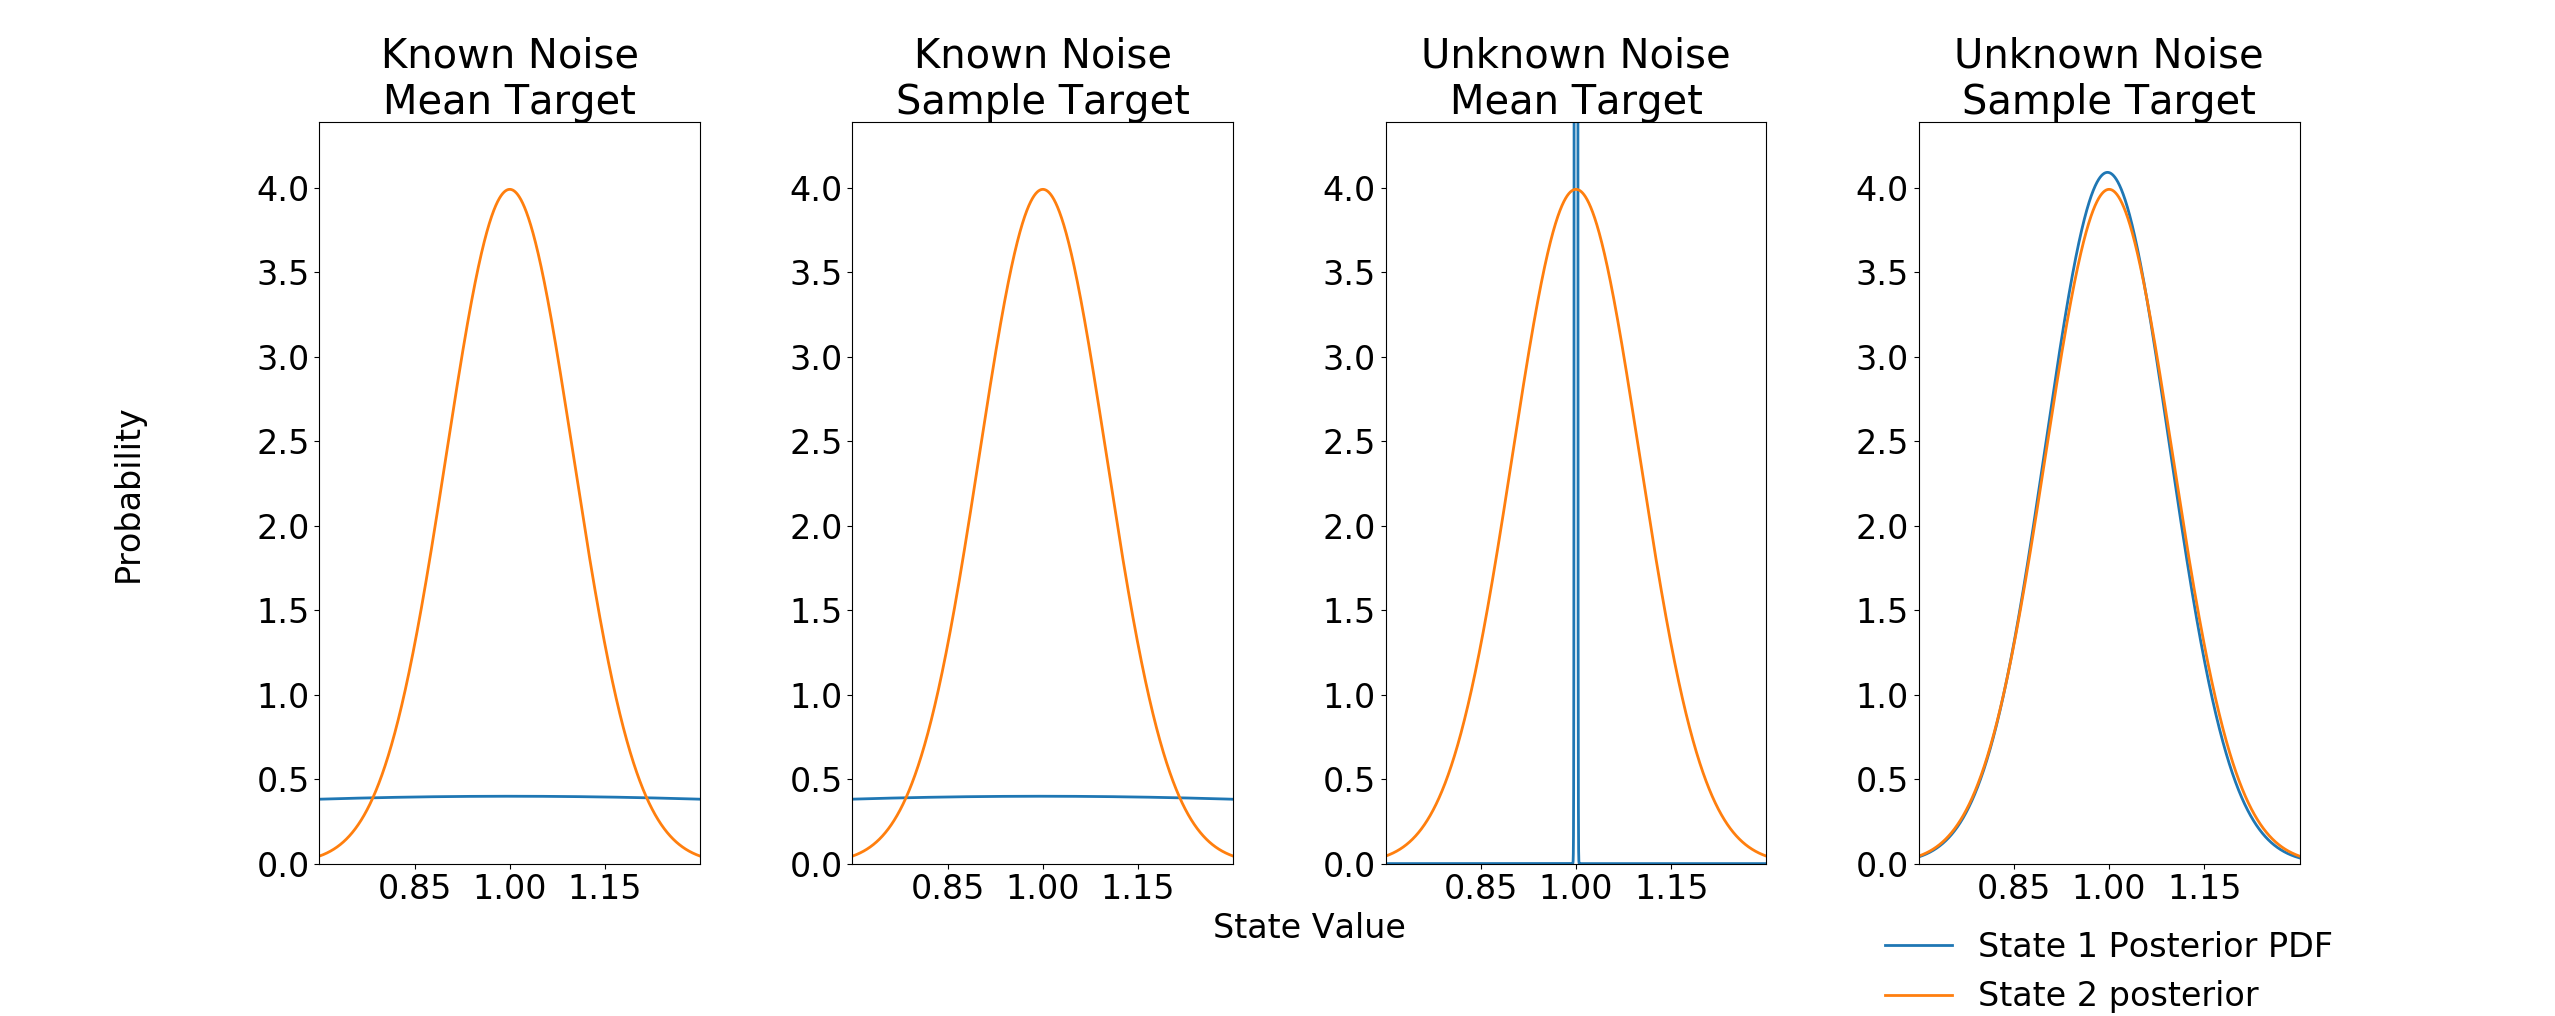
\includegraphics[width=0.6\textwidth, height=0.15\textheight]{1000iterationsSD01.png}
    }
    \\
    \subfloat[$N(1,1^2)$]{
        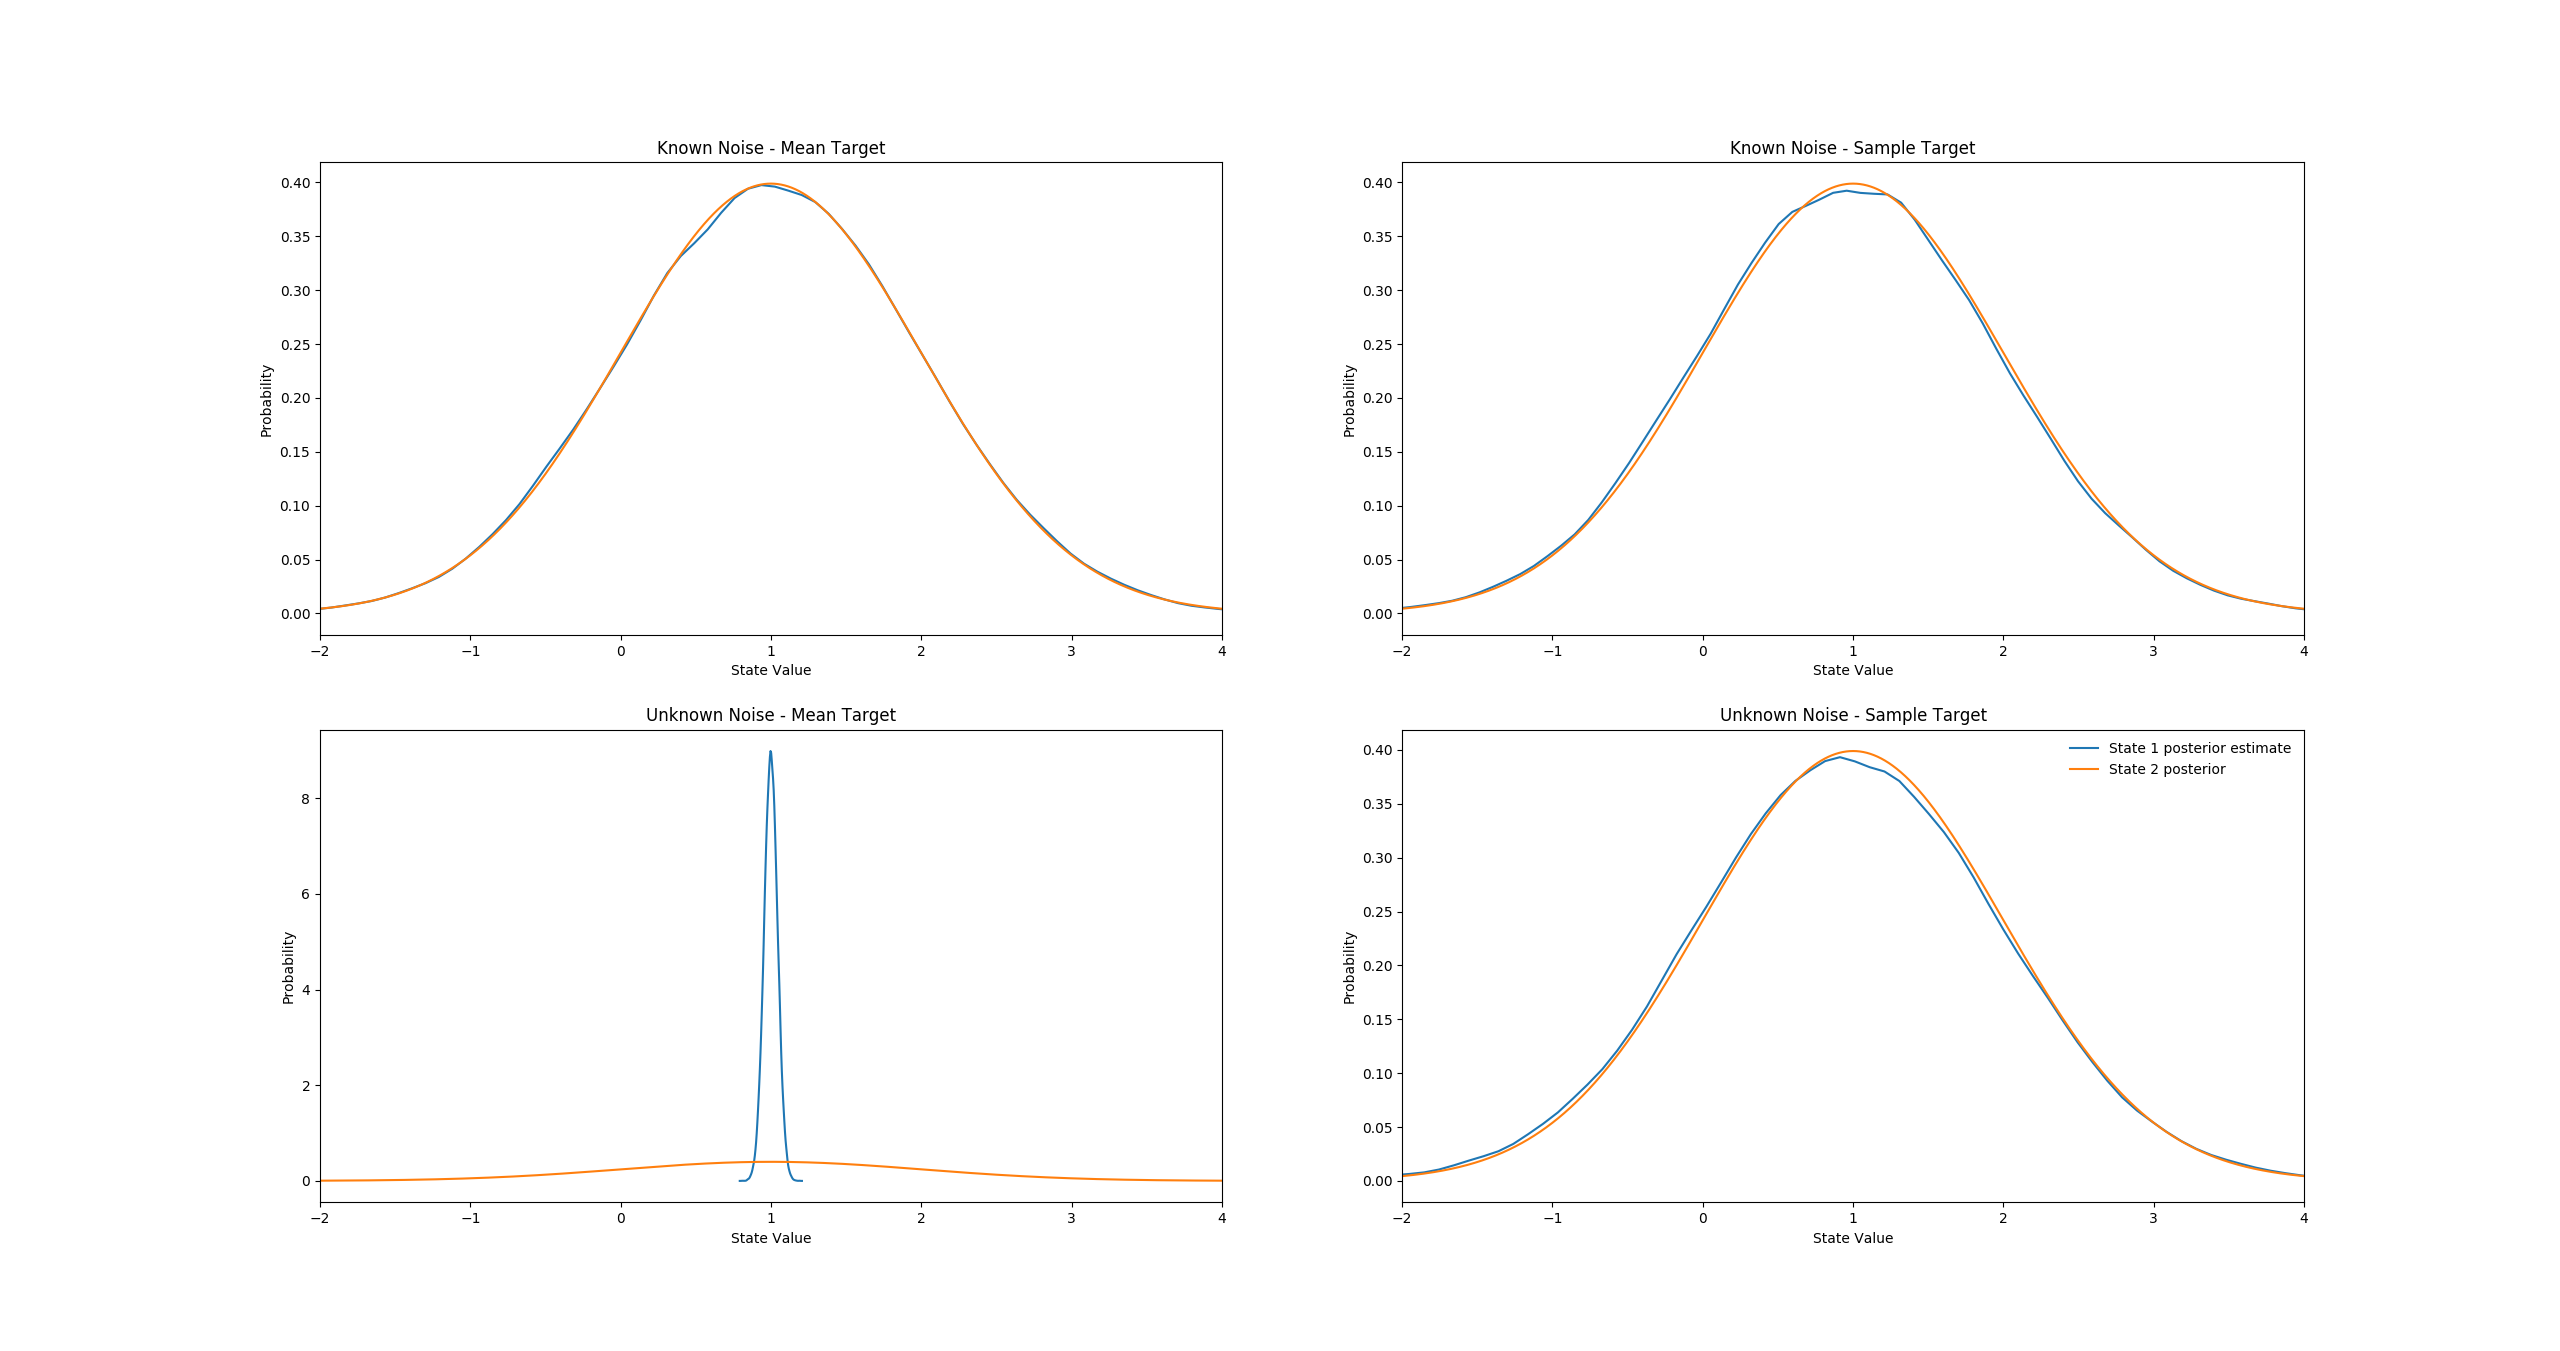
\includegraphics[width=0.6\textwidth, height=0.15\textheight]{1000iterationsSD1.png}
    }
    \\
    \subfloat[$N(1,10^2)$]{
        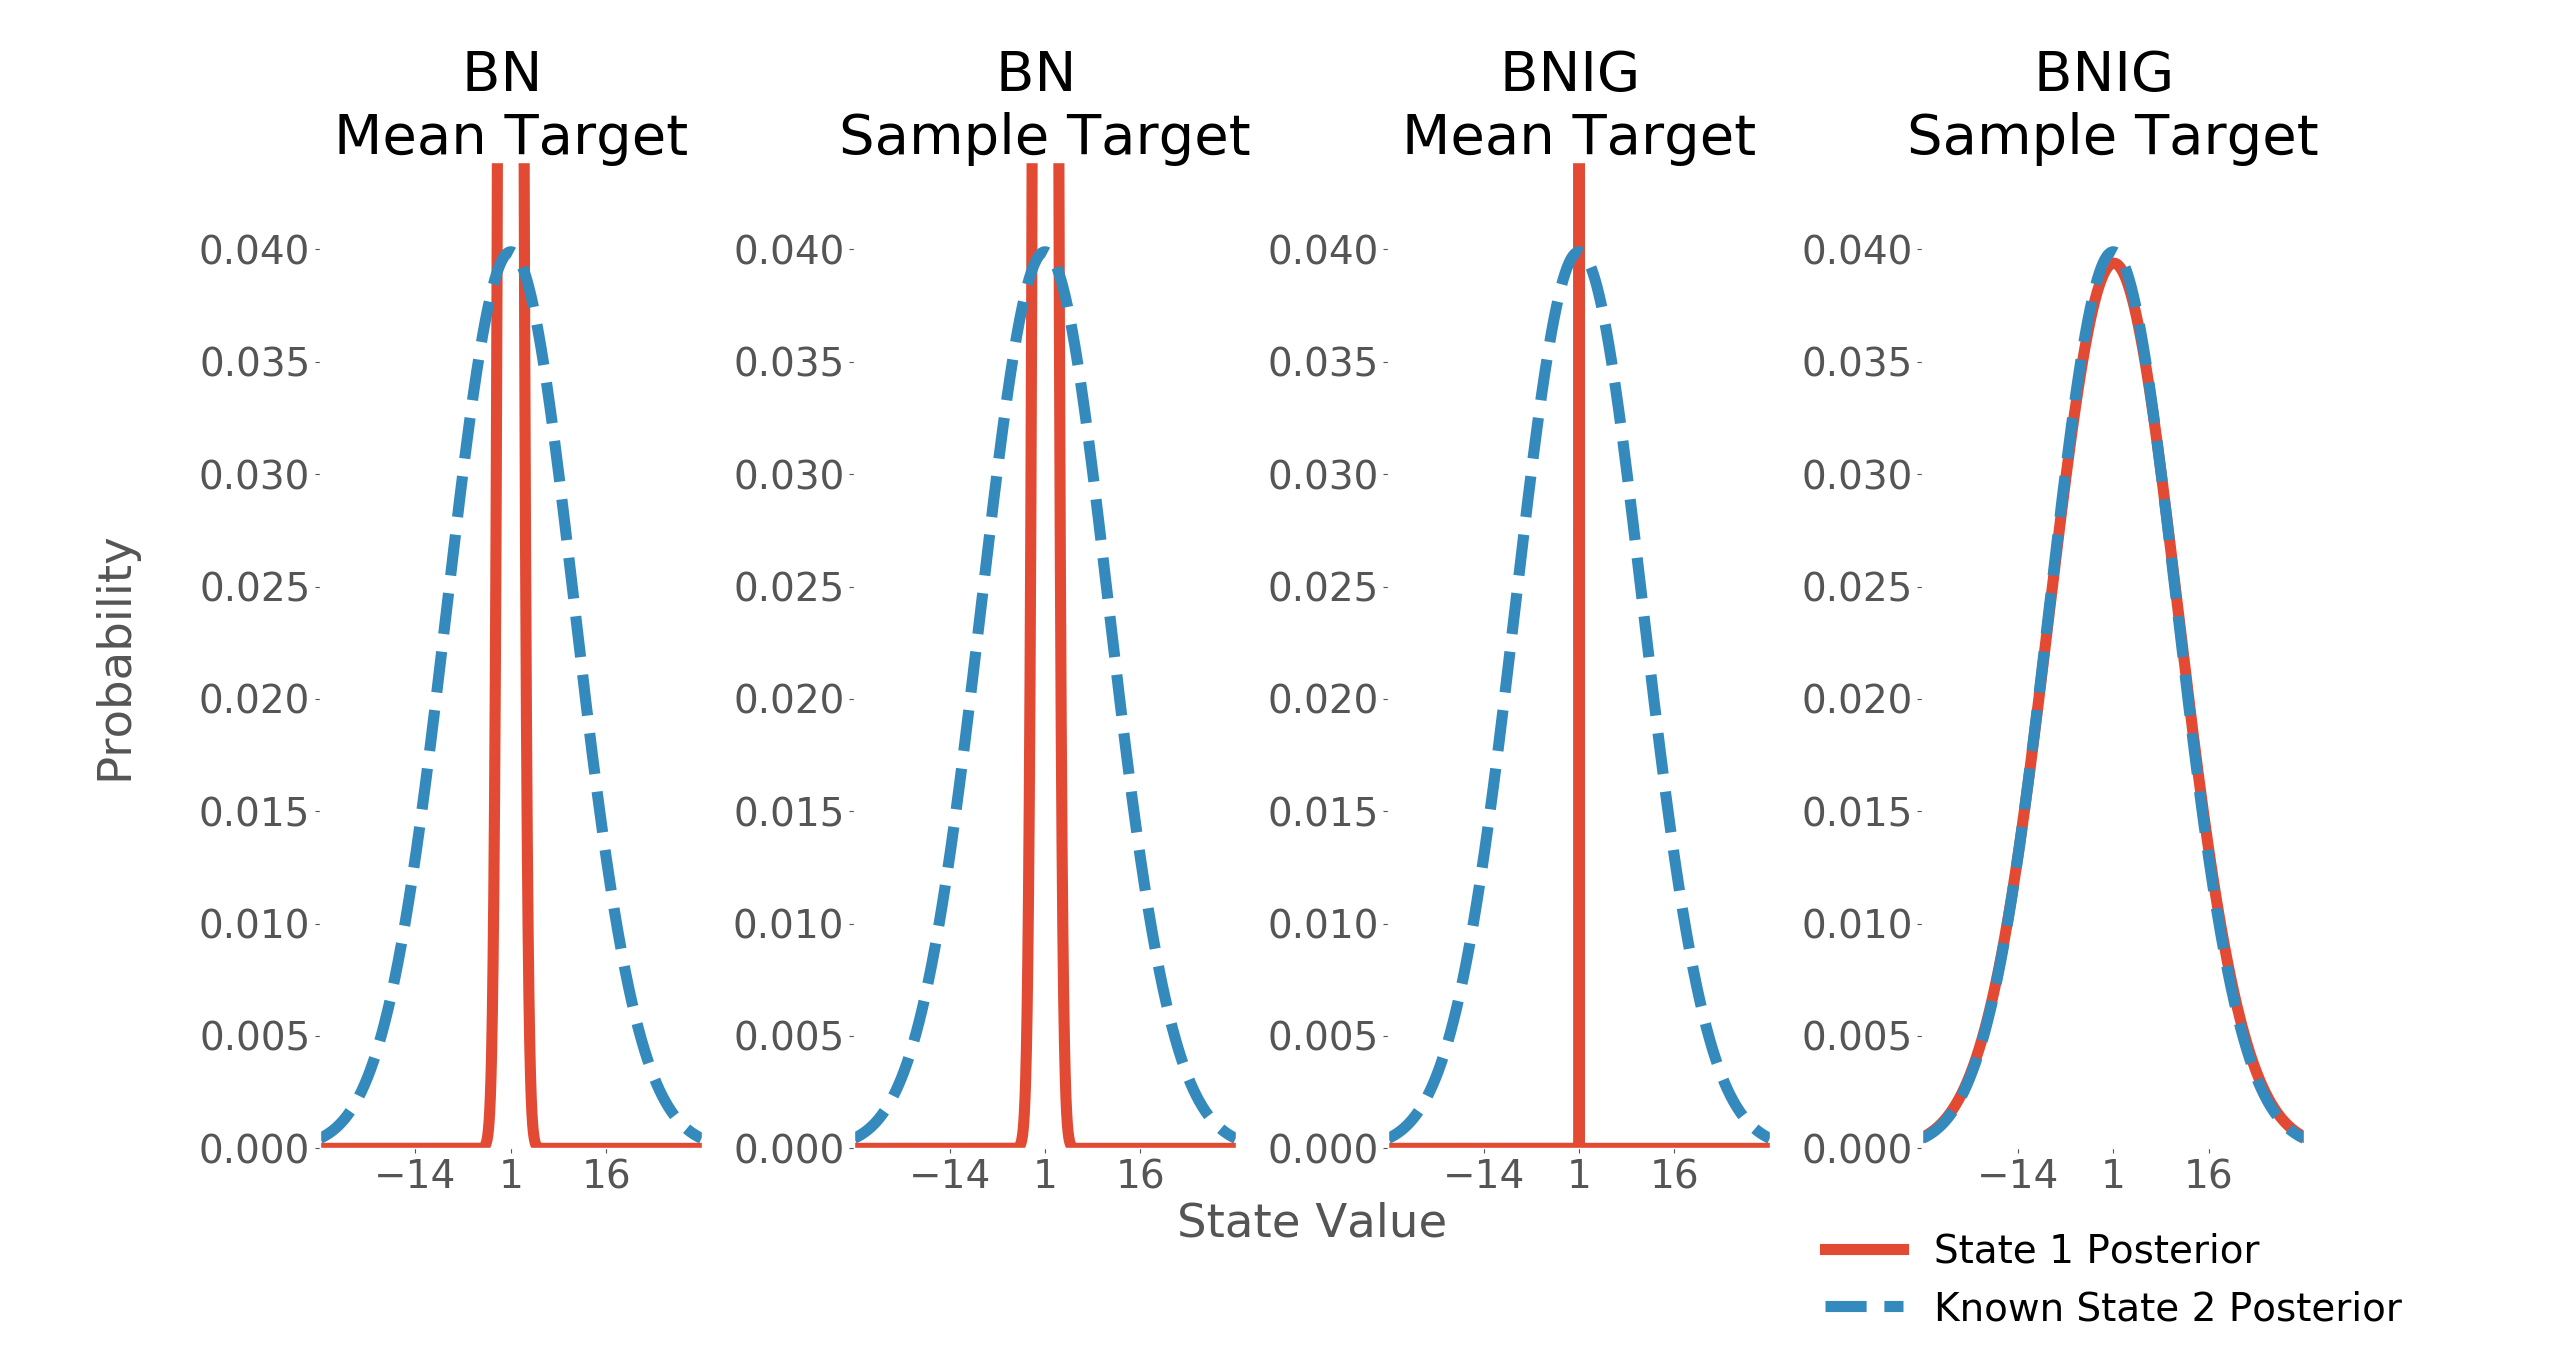
\includegraphics[width=0.6\textwidth, height=0.15\textheight]{1000iterationsSD10.png}
    }
    \caption{\textbf{Variance Propagation On 2 State Toy Example}: The blue lines show the models Q-value posterior distribution while the orange lines show the target posterior distribution. Only the BNIG model with sample targets is able to correctly estimate the target in all cases.}
    \label{fig:proptest}
\end{figure}

The results summarized in figure \ref{fig:proptest} showed that all models were able to correctly estimate the mean. However the target variance was only correctly estimated by the the BNIG model with sample targets. The BNIG model with the MAP target leads to the correct mean but dramatically understimates the variance. This would be an expected result if the model is approximating $\mathbb{E}[Q]$ instead of $Q$. The BN model is only correct for both the mean and sample target if the hyperparameter $\varepsilon$ is set to the correct variance. In an unknown and more complex environment this is unlikely to be possible. However with enough hyperparameter tuning one could argue that this can lead to good results which might explain the results achieved in \cite{azziz_2018}.

Based on these results further developments are focused on the BNIG model with sampled targets.

\section{Variance Propagation}

\subsection{Over Multiple States}

The setting above is in essence a regular regression setting. In a RL setting this variance needs to be propagated to further states. To test that this is still the case with the unknown noise model consider a modification to the environment where an extra state is placed between the initial and terminal state. This state has the same dynamics as earlier. It deterministically transitions to the next state with zero reward over the transition. The correct posterior for each state is then the target posterior in the terminal state. 

The same priors as earlier are used on 4 different target posteriors. The results are summarised in figure \ref{fig:3stateproptest}.

\todo Add details around these experiments in the appendix

\begin{figure}[H]
    \centering

    \subfloat[$N(1,1^2)$]{
        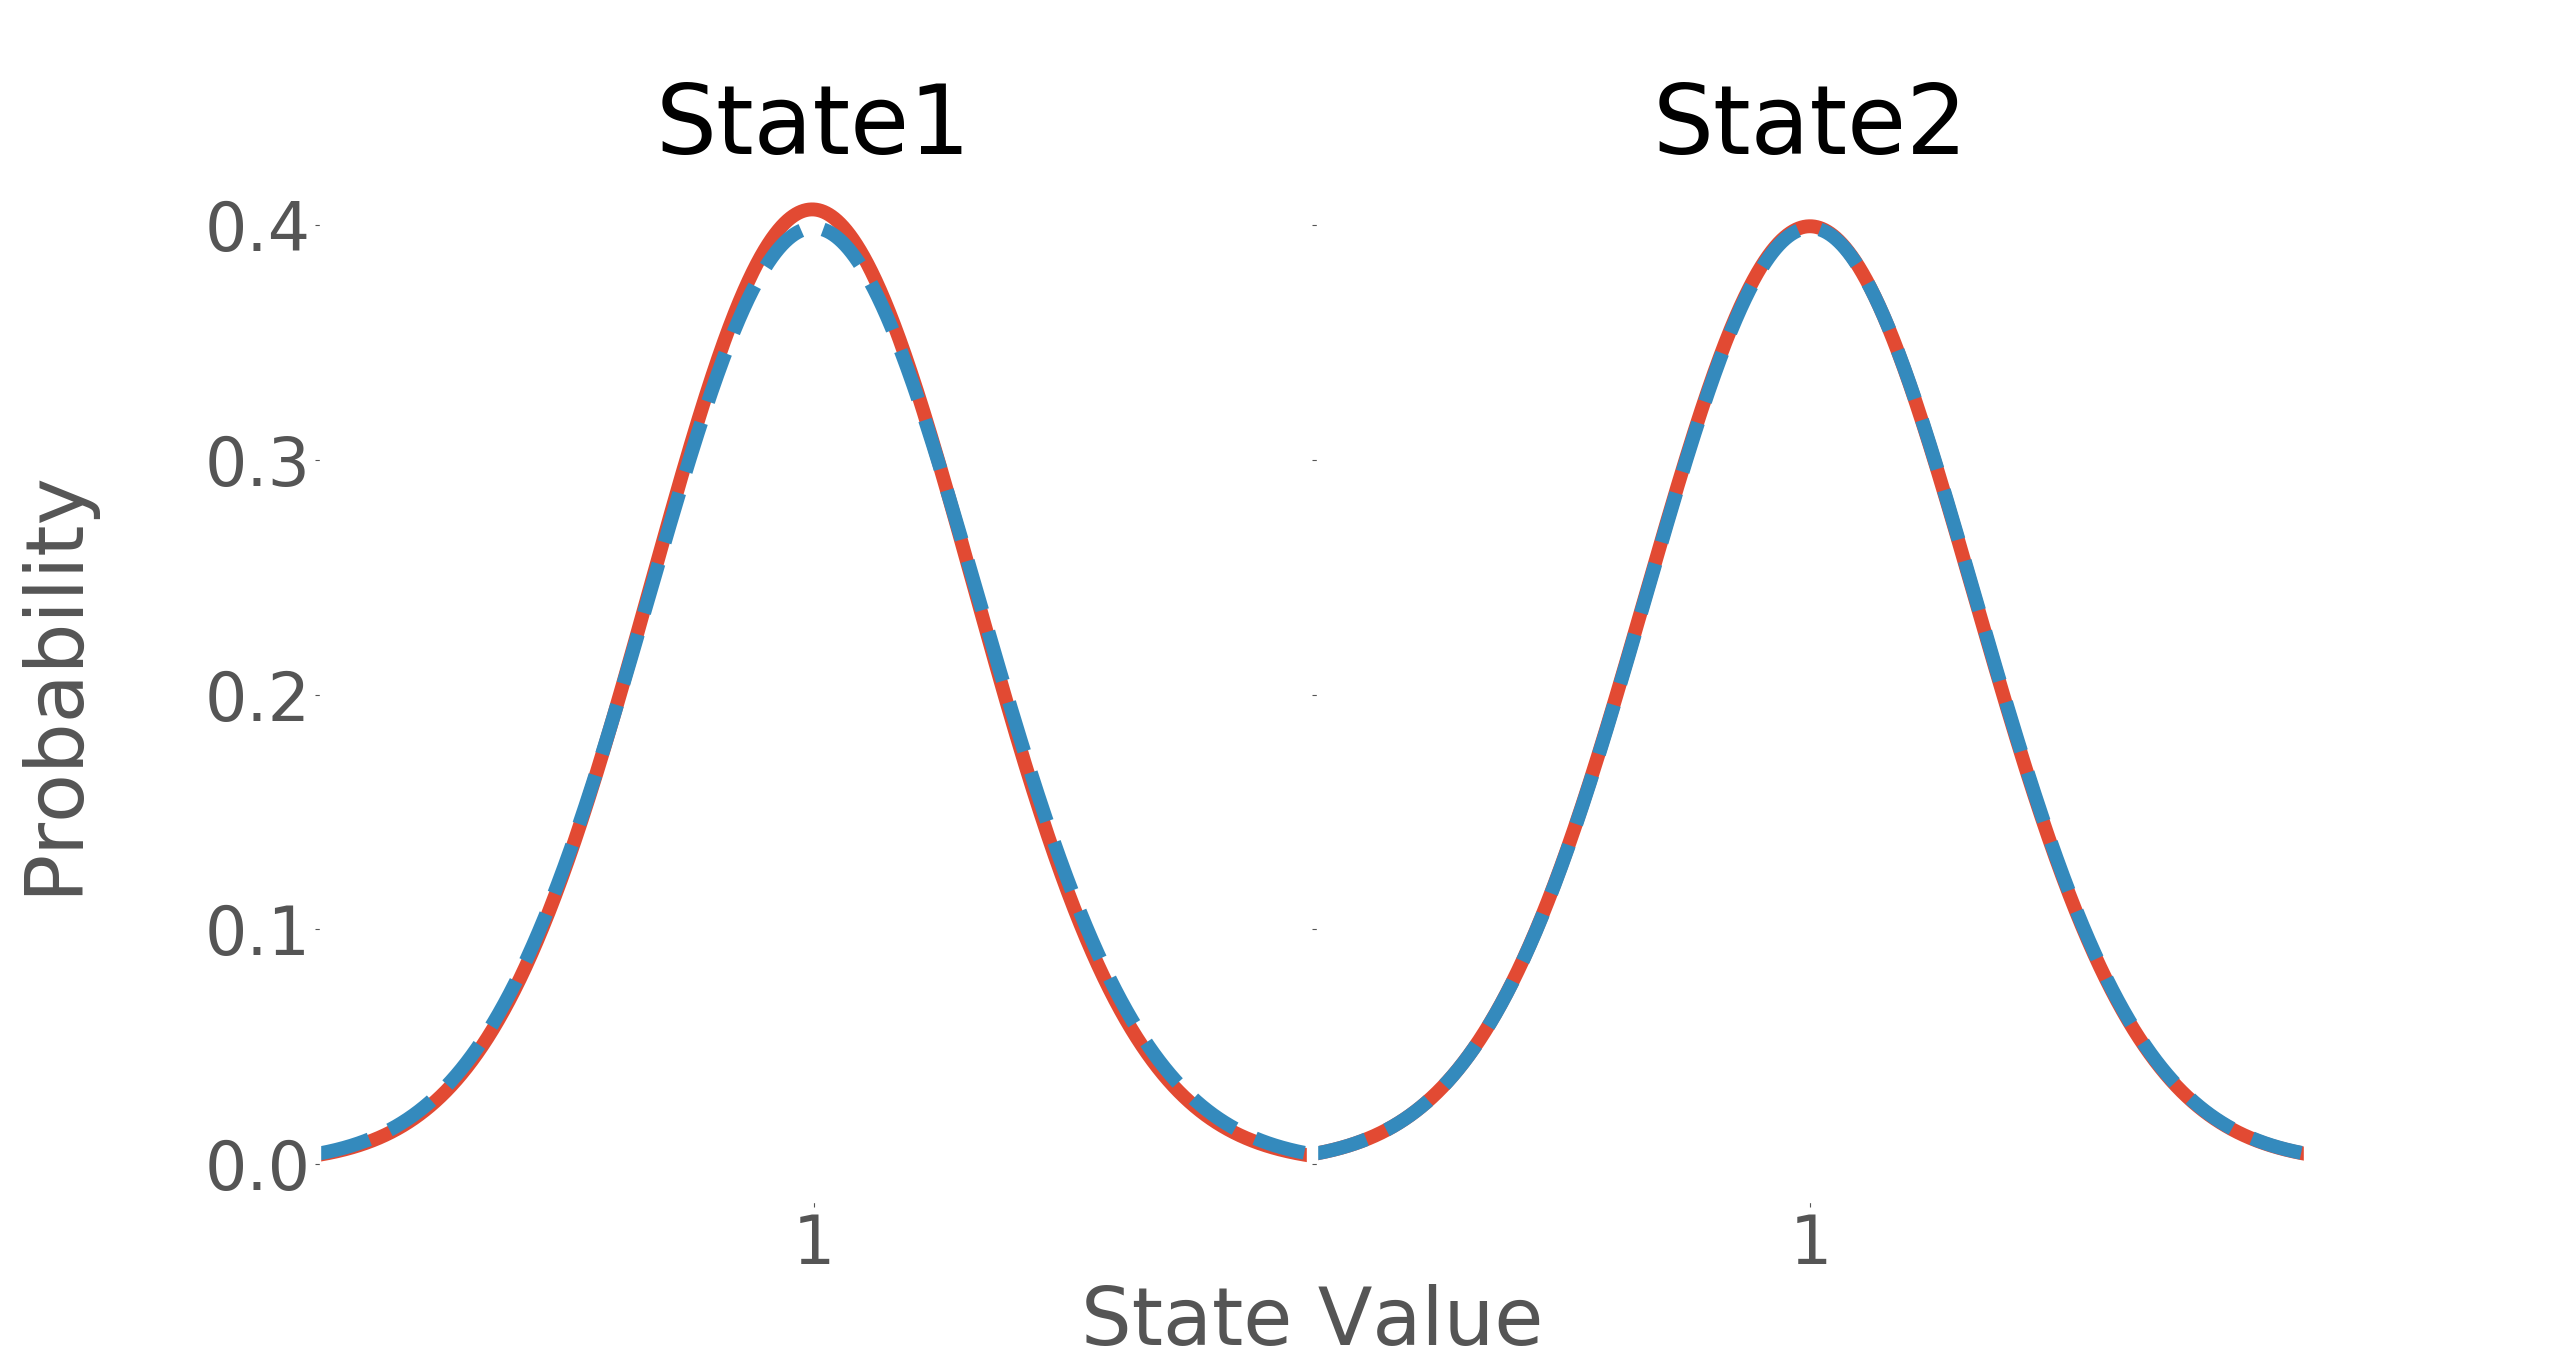
\includegraphics[width=0.45\textwidth]{3State10000iterationsSD1.png}
    }
    \subfloat[$N(1,10^2)$]{
        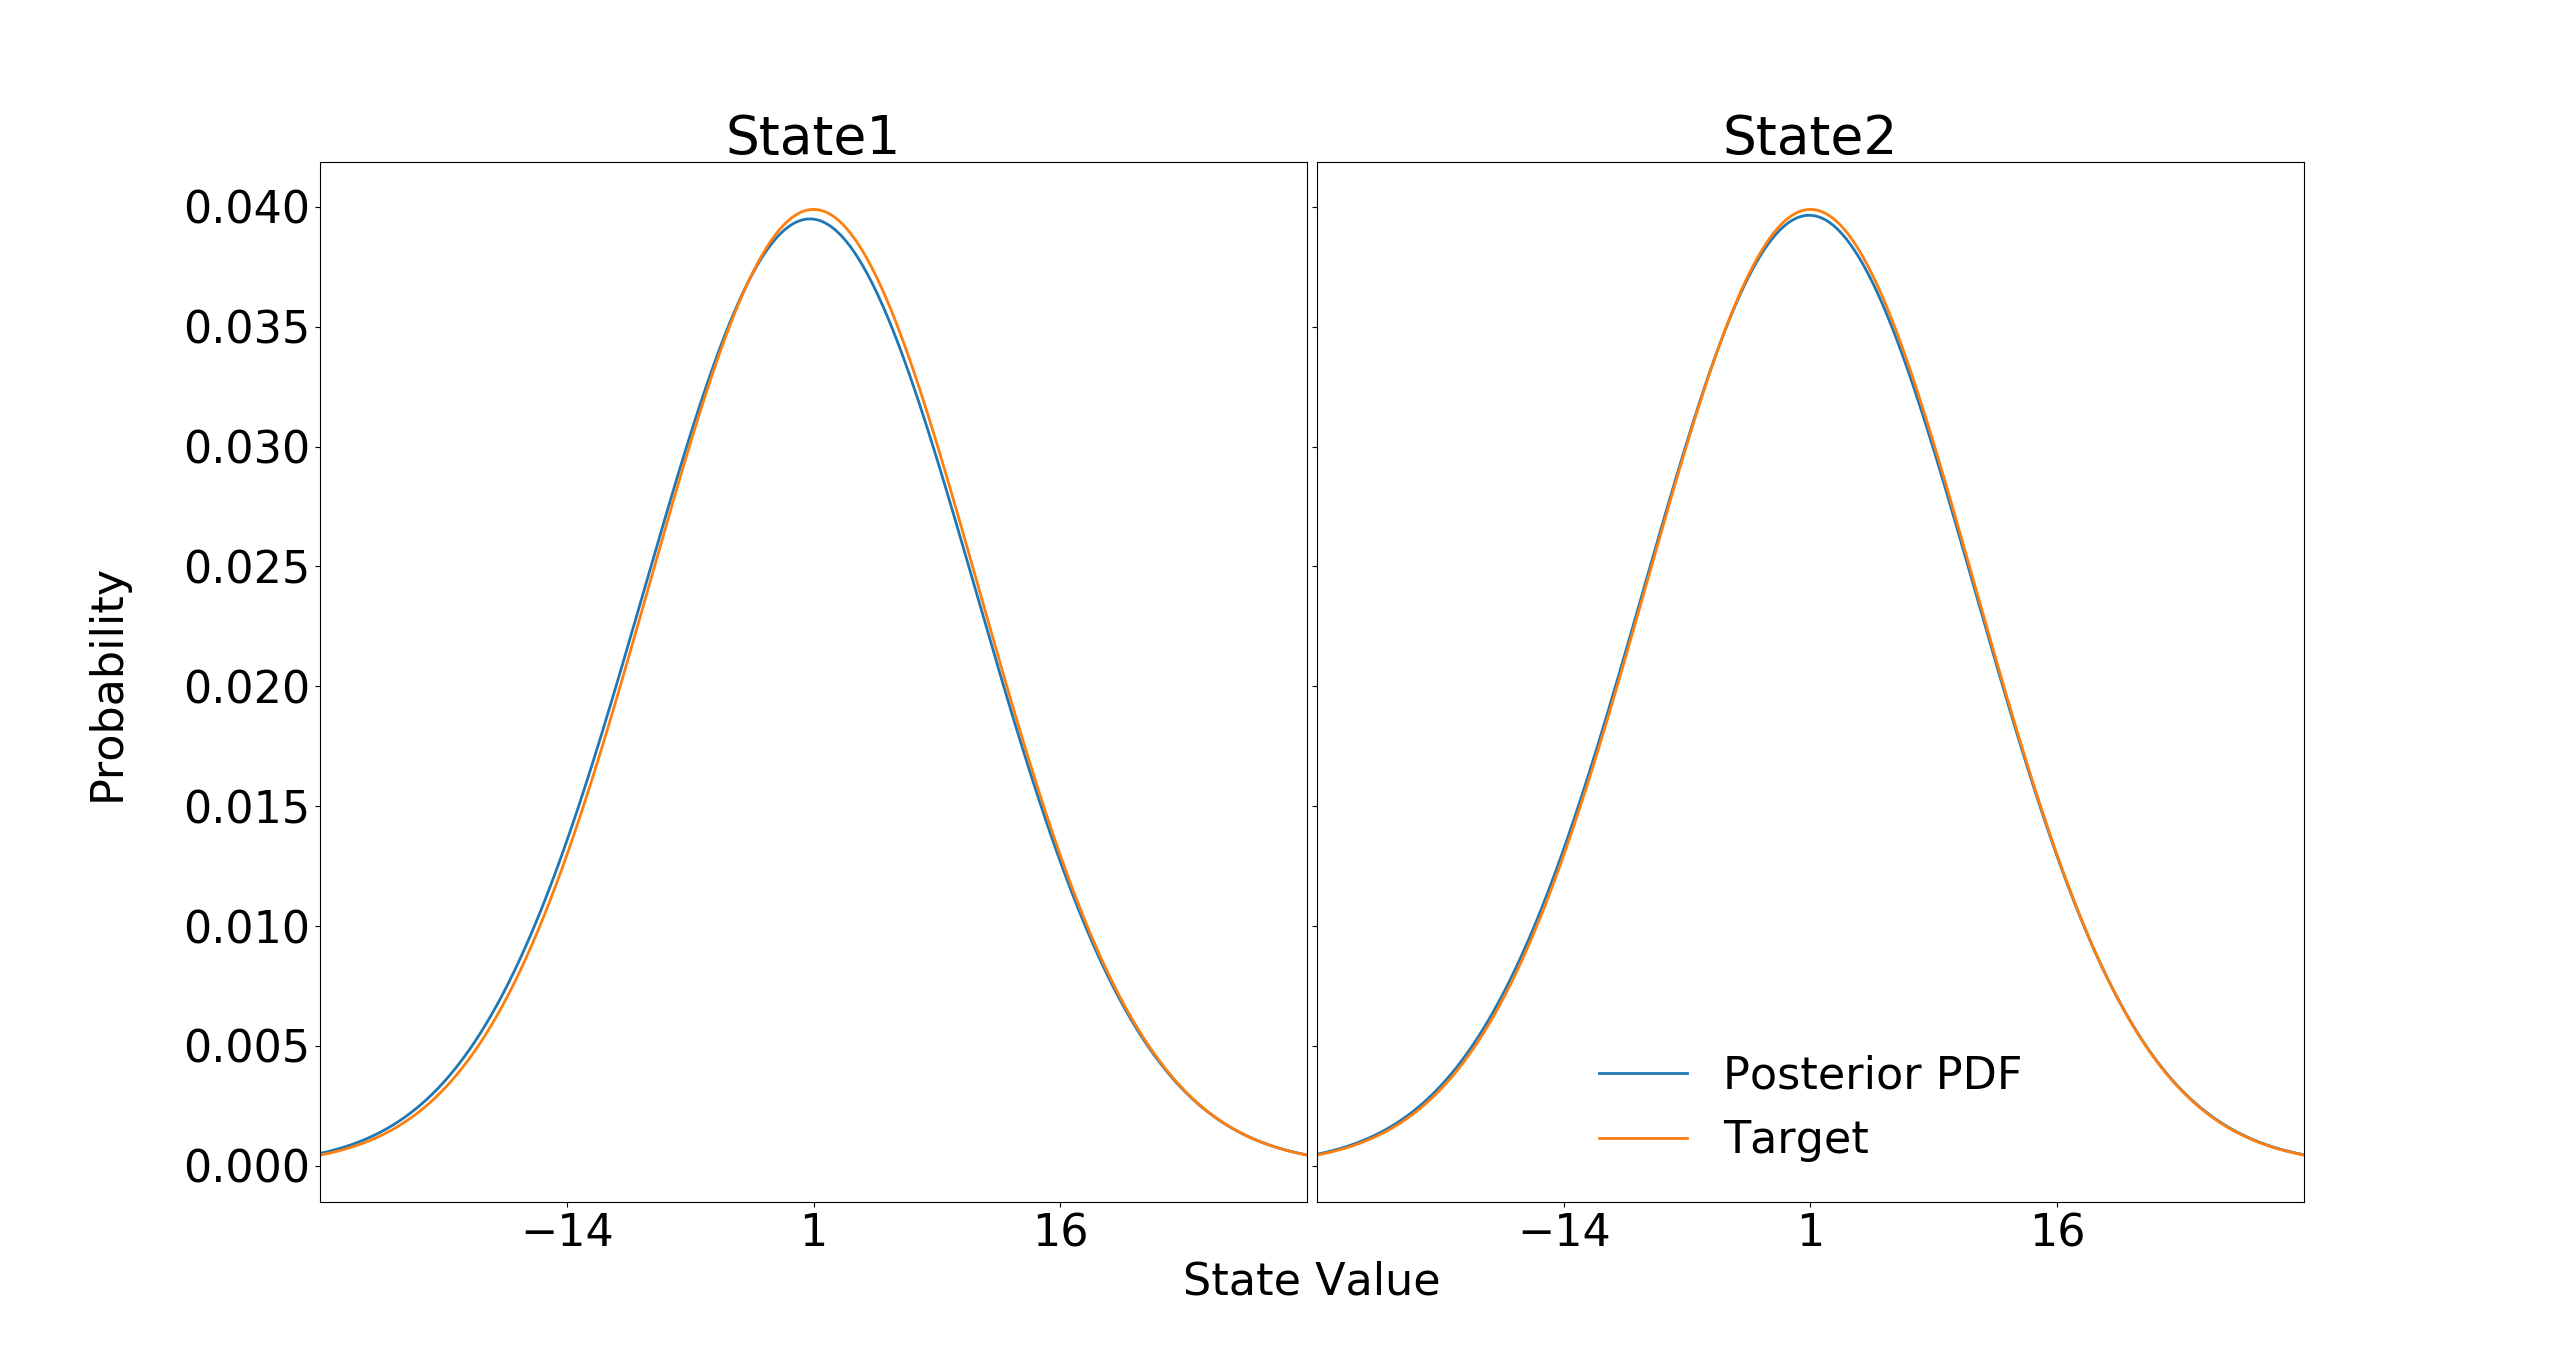
\includegraphics[width=0.45\textwidth]{3State10000iterationsSD10.png}
    }
    \\
    \subfloat[$N(1,0.1^2)$]{
        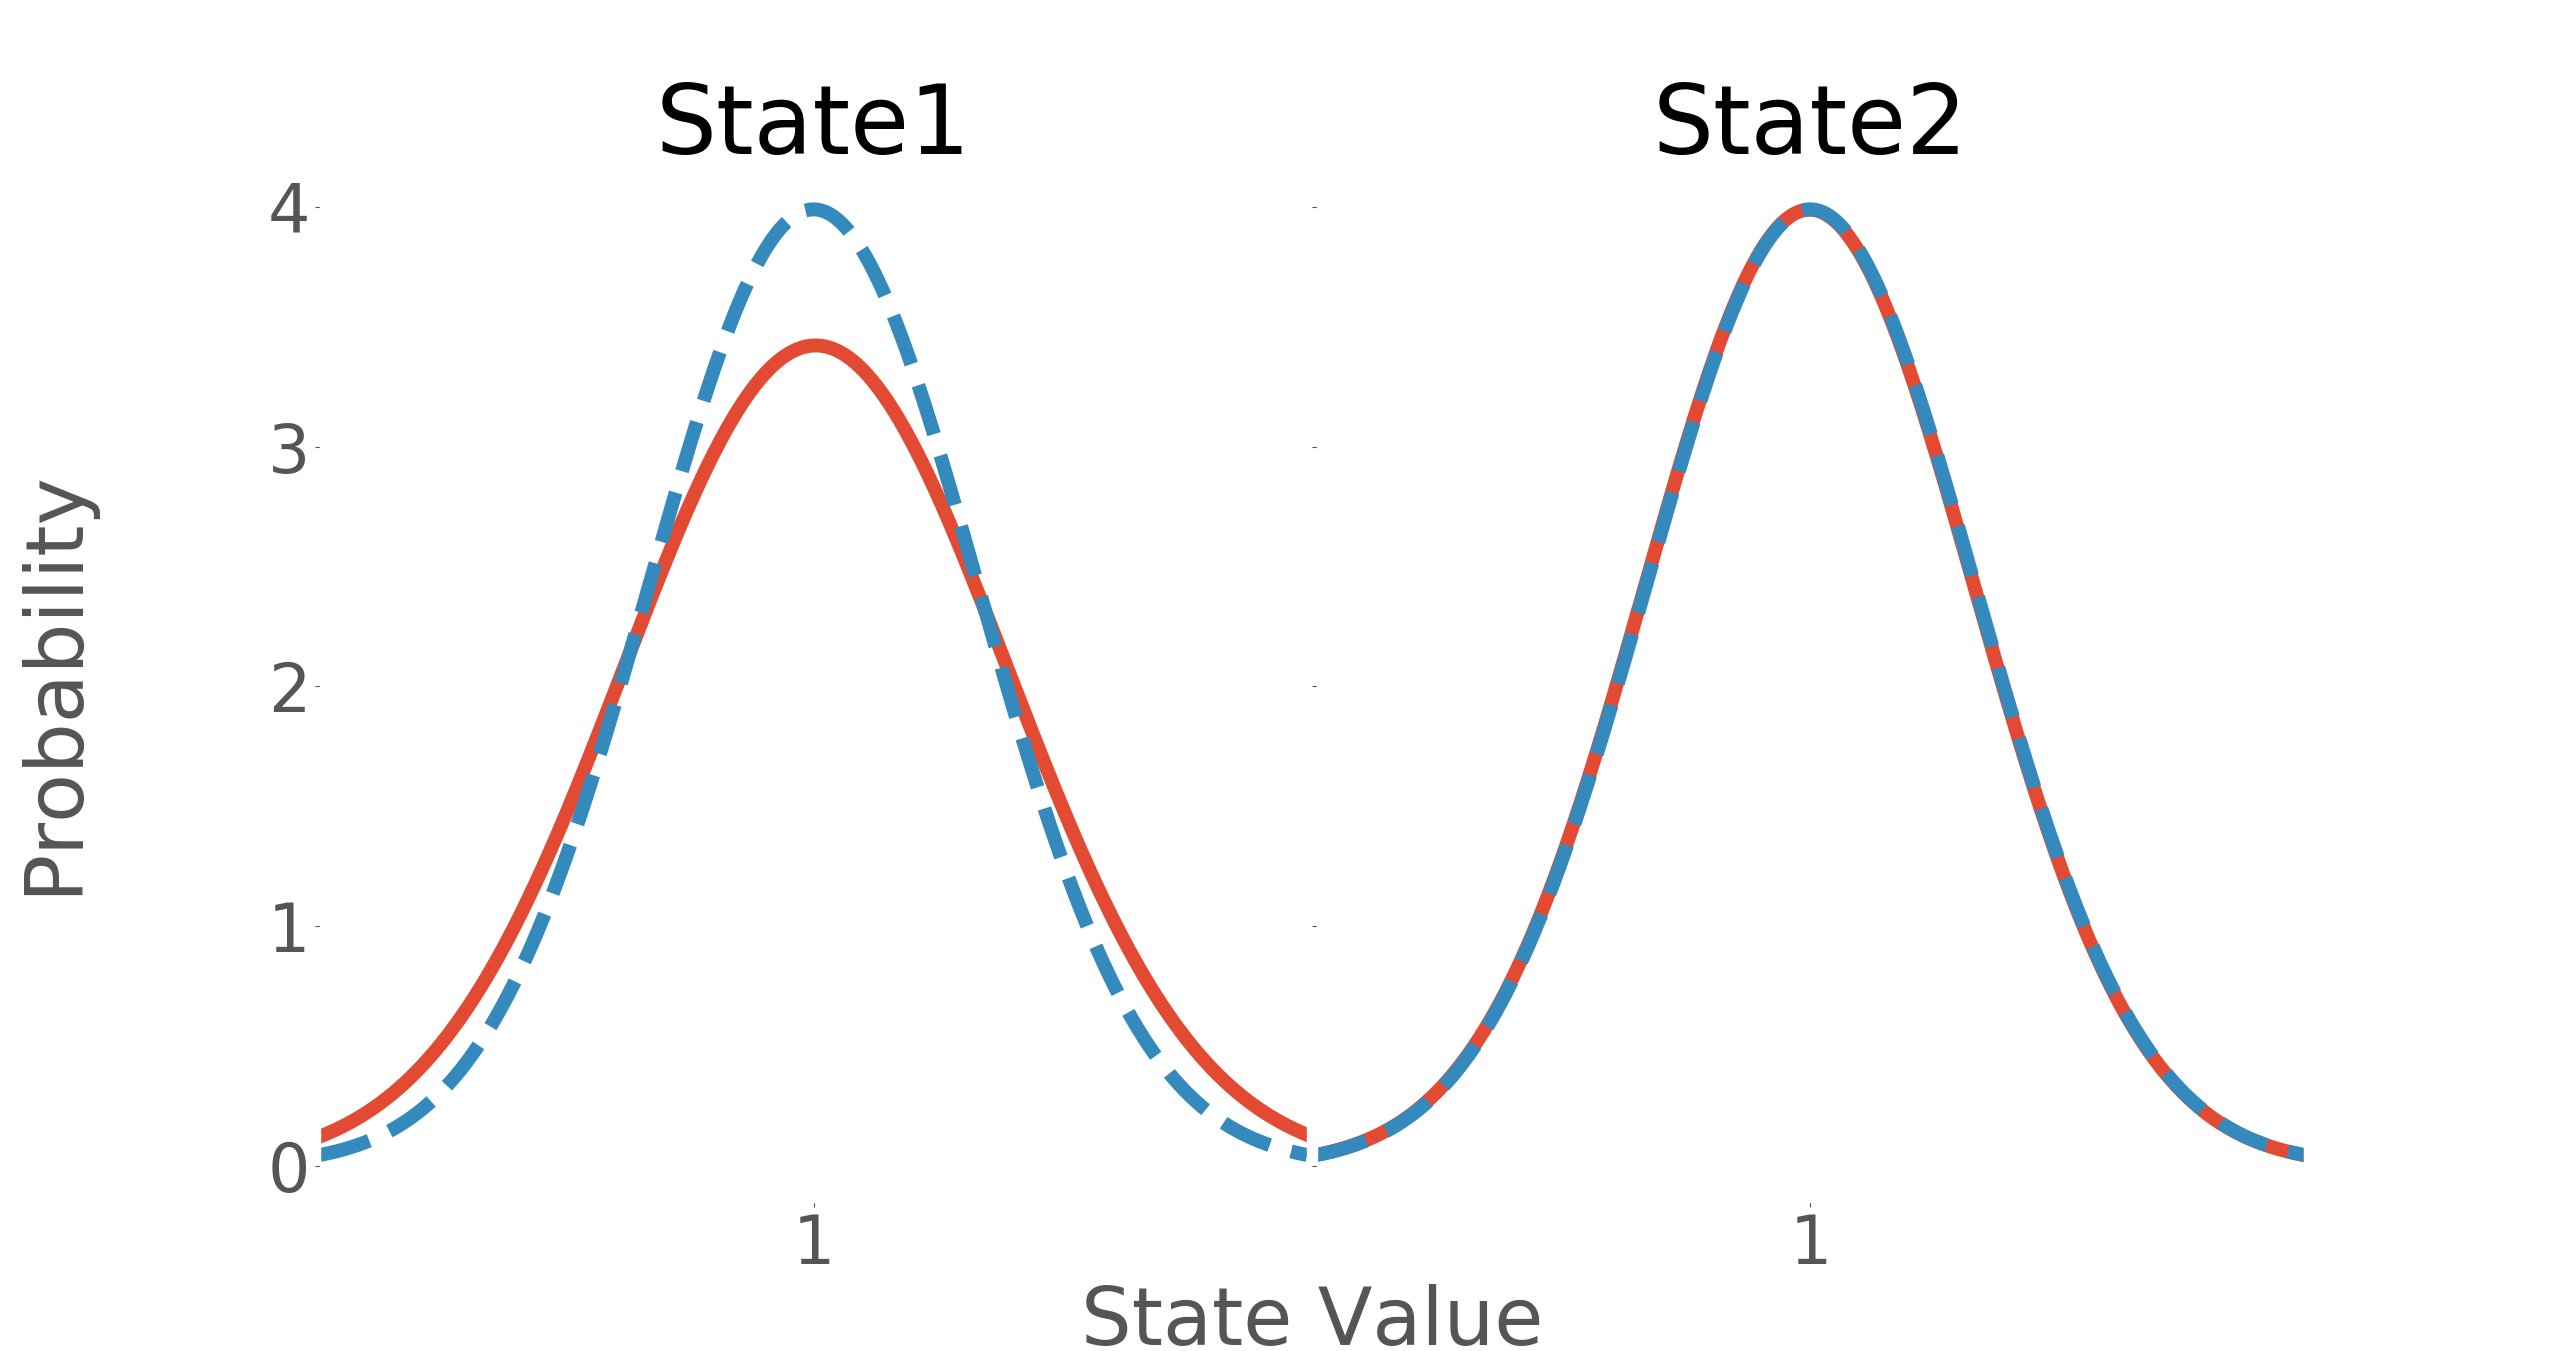
\includegraphics[width=0.45\textwidth]{3State10000iterationsSD01.png}
    }
    \subfloat[$N(1,0.01^2)$]{
        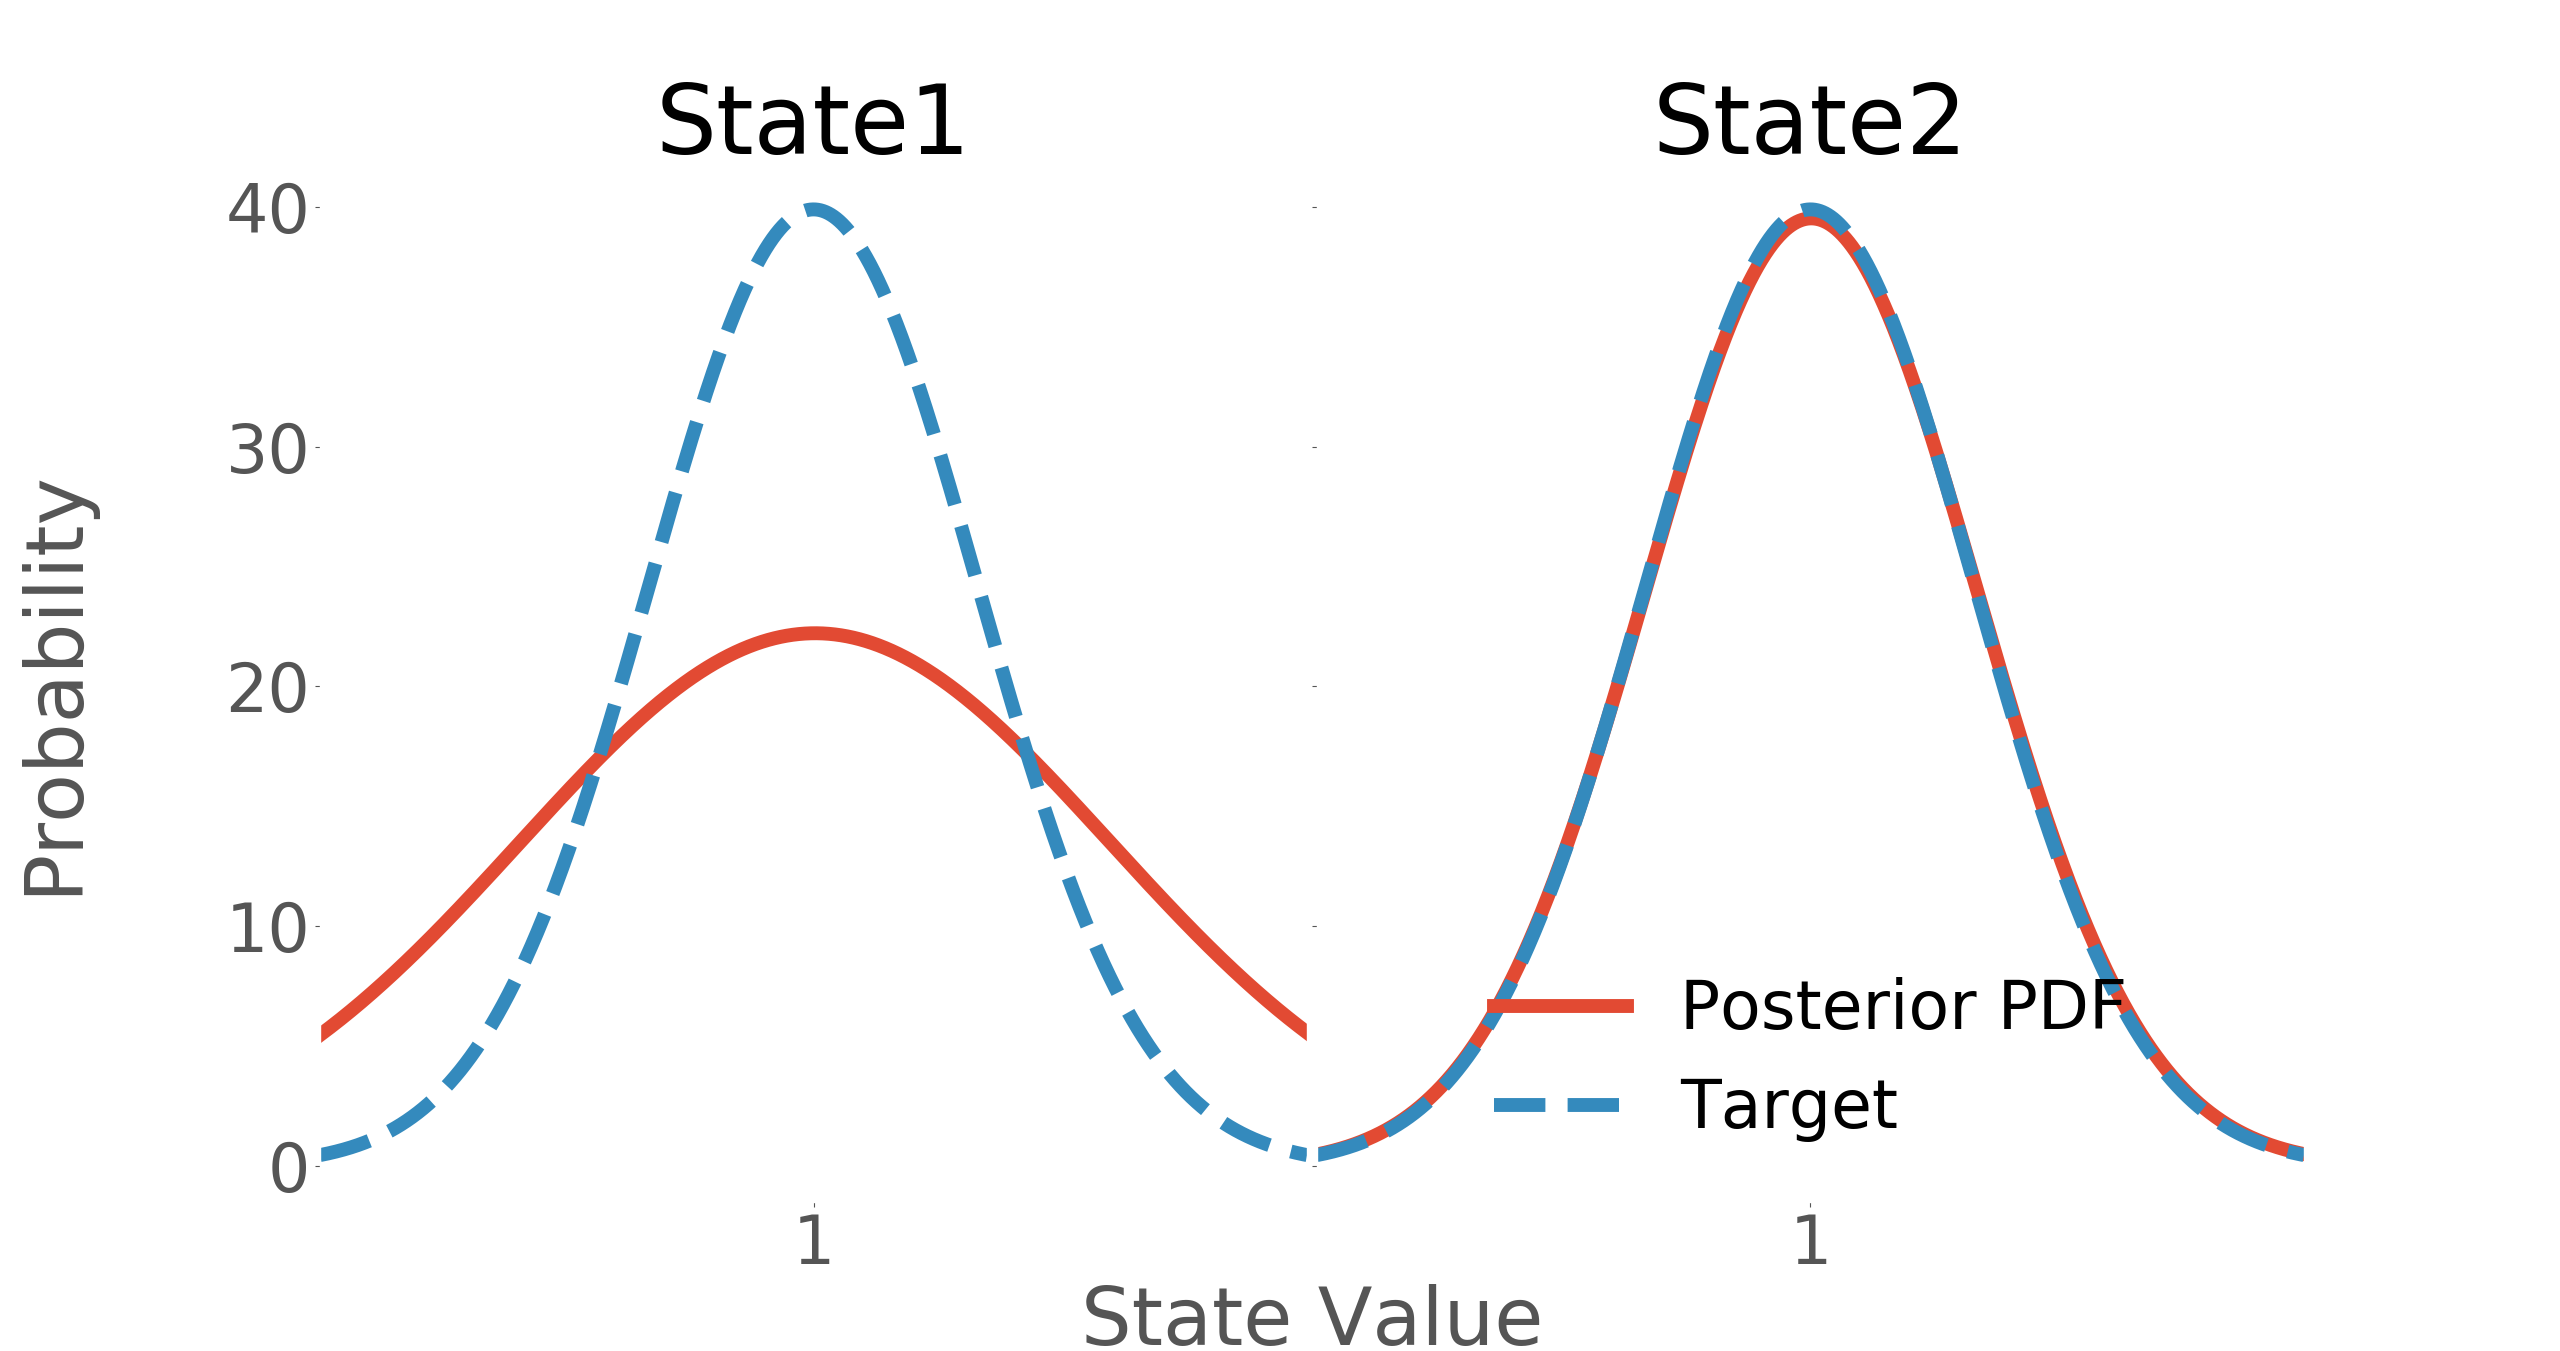
\includegraphics[width=0.45\textwidth]{3State10000iterationsSD001.png}
    }
    \caption{\textbf{Variance Propagation On 3 State Toy Example}: The models posterior estimate for the two first states are shown. The third state is the terminal state that returns a sample from the target distribution.}
    \label{fig:3stateproptest}
\end{figure}

Figure \ref{fig:3stateproptest} shows that for larger variance targets the propagation correctly updates the state 1 variance. However the low variance targets results in an overestimation over the variance in state 1. Running this experiment for more iterations does lead to a better approximation implying that the problem lies in the the convergence rate for different posteriors. 

One possible reason for this is that the posterior representing the 0.01 standard deviation posterior is more sensitive to small changes in in its parameters than the larger variance posteriors. In other words small changes in the parameters for a distribution with low variance leads to large changes in the variance of the posterior. Since the learning is happening in an online fashion the first estimates of the posterior will likely have large error. This effect is amplified for state 1 since it is training on the large error state 2 posterior. (\todo: Confirm/source that this is actually the case)

By extending the toy example to even more states as in figure \ref{fig:longproptest} one can see that this problem increases the further the variance needs to be propagated. Even large variance targets will fail to correctly propagate given enough states.

\begin{figure}[H]
    \centering
    \subfloat[6 States with $N(0.1,1^2)$]{
        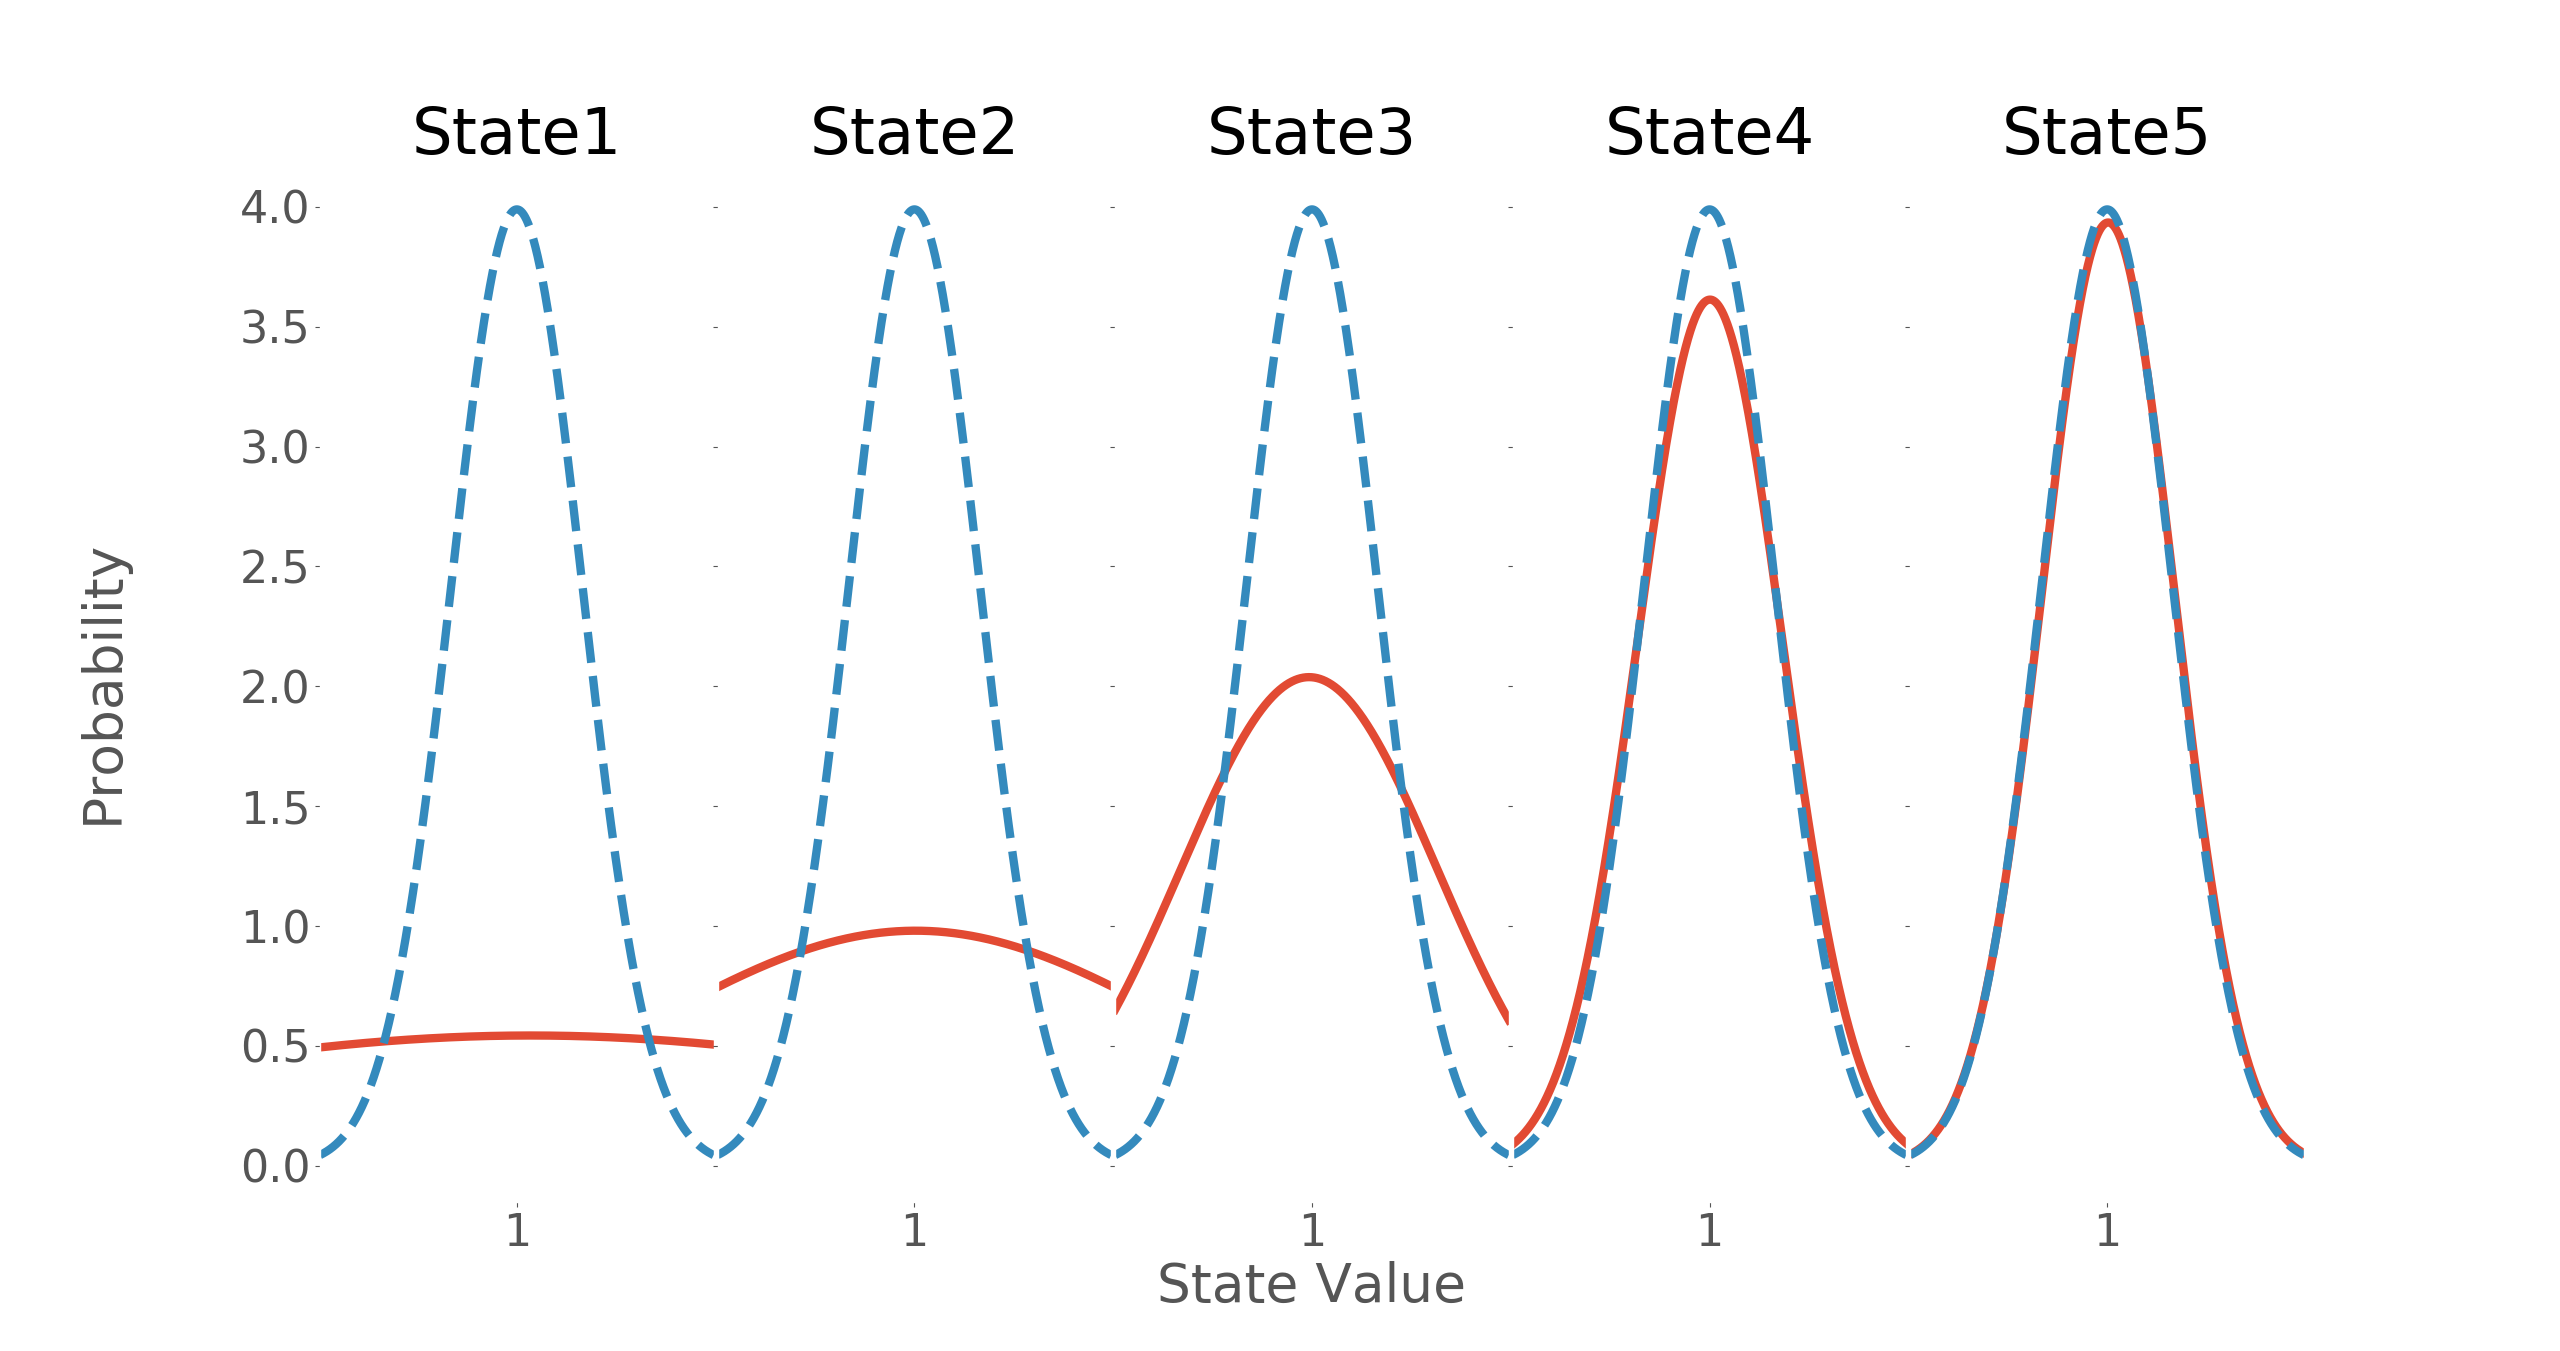
\includegraphics[width=0.7\textwidth]{6State1000iterationsSD01.png}
    }
    \\
    \subfloat[6 States with $N(1,1^2)$ target]{
        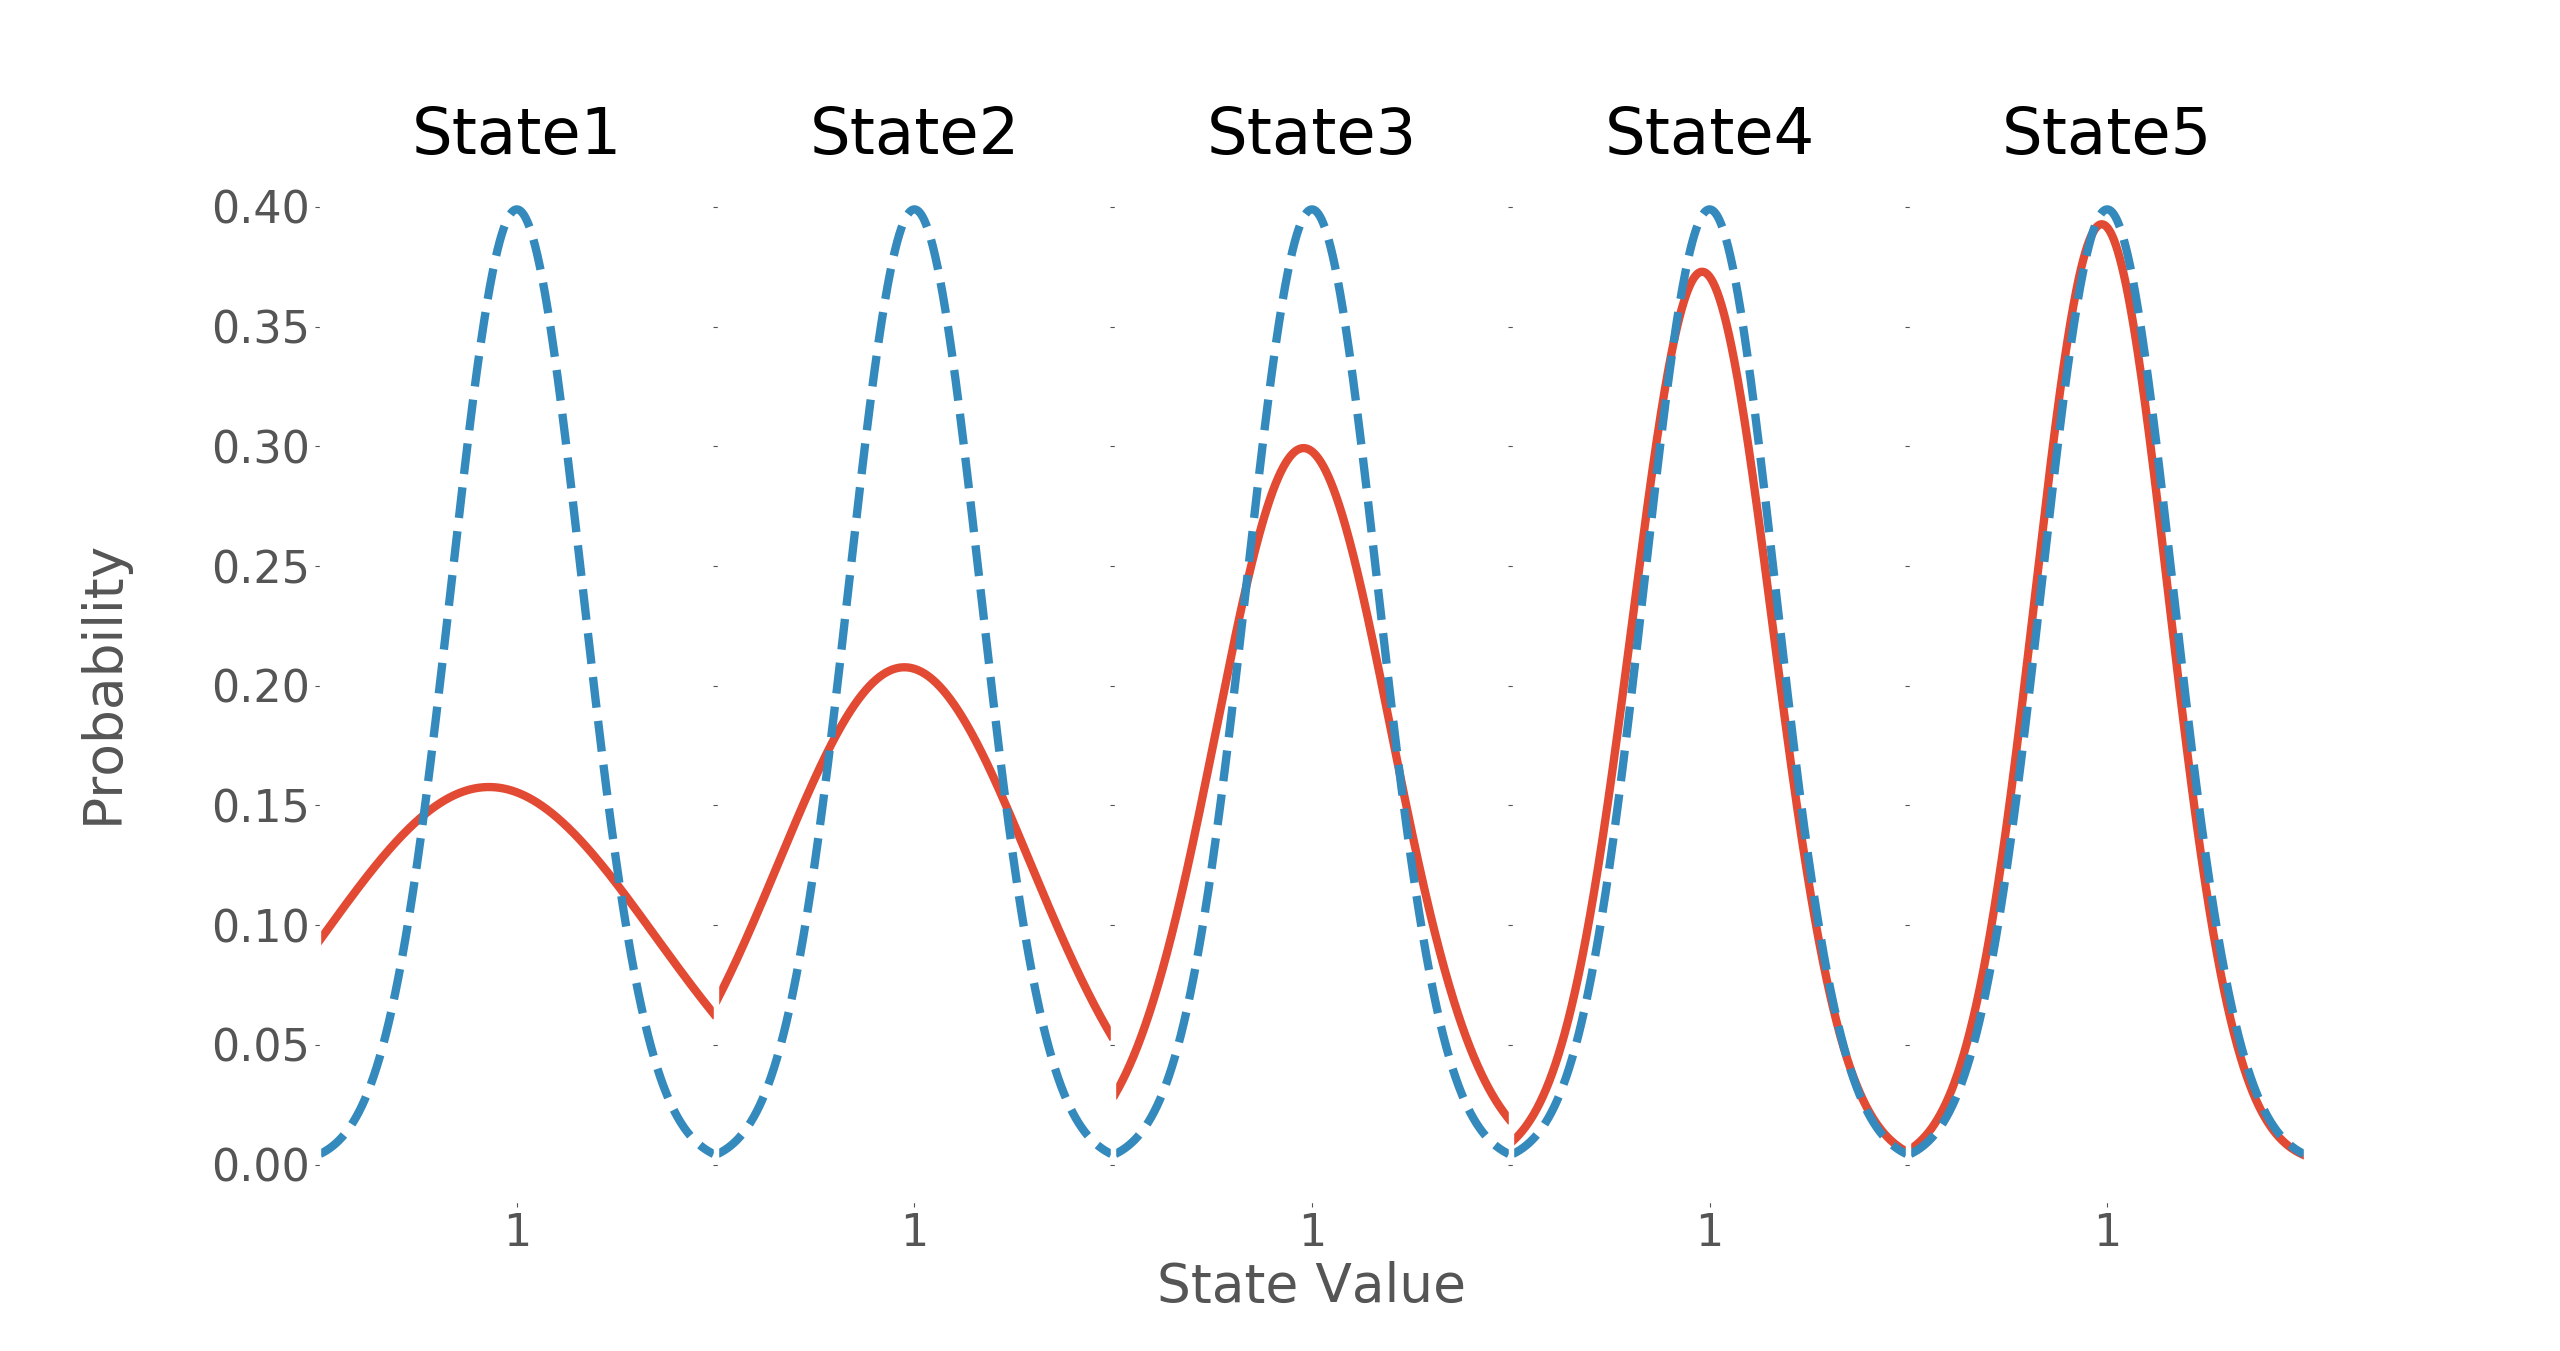
\includegraphics[width=0.7\textwidth]{6State1000iterationsSD1.png}
    }
    \caption{\textbf{Failure of variance propagation over many states}: (\textbf{a}) shows that the error in estimation close to the terminal state leads to failure in the estimation of the posterior of the initial states. In (\textbf{b}) the seemingly correct estimation close to the terminal state still does not prevent errors Closer to the initial state.}
    \label{fig:longproptest}
\end{figure}

This issue will be refered to as the speed of propagation. It encompasses the problem of quickly propagating variance estimates from downstream states back to states which are far from the environments reward.

\todo: Define speed of propagation. Maybe a seperate subsection that plots how the error changes with length of chain. How do we measure the error between two distributions? KL Divergence?

\subsection{Speed of propagation}

Inorder to improve the speed of propagation insight is required into what causes the issue. In this section two causes and methods for counteracting them are discussed. However these are not necessarily the only two causes of slow propagation.

\todo These argumentations are weak and require sources or "proof". 

The first cause is best explained using an example. Consider the 3 state toy example. State 1 can only converge to the correct distribution once State 2 has converged. If more states are added, State 1 will converge once all the states between it and the terminal state have converged. The longer the chain is, the more iterations are required for state 1 to converge. This issue is the same issue faced with the expected Q value in regular RL which is dealt with through a bias-variance trade-off (\todo Include n-step in theory). Similarly extending the 1-step update to an n-step update one will increase the speed of variance propagtation with the downside of introducing more variance to the $\sigma_\varepsilon$ estimate.

The second cause is a result of no longer using a step size when updating the Q-values using bayesian updates. In regular Q-learning the step size can be viewed as the weighting of new data relative to the current model. This effect is also found in the bayesian setting in the posterior update that combines the prior and the new data. However, in regular Q-learning the step size also leads to the model forgetting old data(\cite{sutton_barto_2018}\todo find this page). This does not happen in the bayesian regression setting that has been used.

In the bayesian regression setting described the prior is always the previous posterior. In simple terms the model assumes all data to be equally important. Recalling that the prior used is the previous posterior, a prior based on many datapoints will have a bigger impact on the posterior than a single new datapoint. This is a problem since a reinforcement learning problem is almost always non-stationary. With this weighting scheme the new data points which are more relevant to the current target are weighted the same as a datapoint collected based on the initial priors.

Counteracting this effect while retaining the bayesian regression model is not trivial. This thesis addresses the problem using the solution described in \cite{azziz_2018} with a slight modification. Define a hyperparameter $T_{bayes}$ and train a new bayesian regression model from scratch using targets from the old model every $T_{bayes}$ steps. This setup is for batch updates, so in this online linear case the priors for $\lambda$, $\alpha$ and $\beta$ are reset while the mean value $\mu_\beta$ is left unchanged. 

\todo Deep exploration?

\section{Performance on Linear RL Problem}

Up to now the model has only been tested on simple problems with known posteriors. To test how well this generalizes to a more realistic RL environment consider a variant on the corridor environment introduced in the theory section in figure \ref{fig:chain}.

Consider a chain of length N where the goal is to move from the initial state on the left side of the corridor to the final state on the right side of the corridor in N steps. A reward of 1 is given in a final state, moving left gives a reward of $\frac{1}{100N}$ and otherwise the agent recieves no reward.

\todo add regret to theory section

The BN, BNIG models was compared with the known noise bayesian model and a linear Q-learning method following an $\varepsilon$-greedy exploration scheme. As in \cite{osband_2018} models were compared by the average number of episodes required to "learn" the enivorment. In this case the enivorment is considered learned when the running average regret of the last 100 episodes drops below 0.1.

\todo plots of results and discussion around these


\cleardoublepage